%\documentclass[12pt]{article}
\documentclass[smallextended]{svjour3}
%
\usepackage[utf8]{inputenc}
\usepackage{graphicx,subfig}
\usepackage{amstext,amsmath,amssymb,bm,bbm,mathtools}
\usepackage[linesnumbered,lined,boxed,commentsnumbered]{algorithm2e}
\usepackage[export]{adjustbox}
\usepackage{array,multirow}
\usepackage[dvipsnames]{xcolor}
\usepackage{amsmath}
\usepackage{amssymb}
\usepackage[
backend=biber,
style=alphabetic]{biblatex}

\DeclareMathOperator*{\argmin}{arg\,min}
\DeclarePairedDelimiter\norm{\lVert}{\rVert}%
\DeclarePairedDelimiter\abs{\lvert}{\rvert}%

\newcommand{\todo}[1]{{\textcolor{blue}{#1}}}
\newcommand{\jaco}[1]{{\textcolor{green!50!black}{#1}}}
\newcommand{\HT}[1]{{\textcolor{violet}{#1}}}
\newcommand{\daniel}[1]{\textcolor{NavyBlue}{#1}}
\newcommand{\R}{\mathbb{R}}
\newcommand{\Z}{\mathbb{Z}}
\newcommand{\Equ}[1]{(\ref{#1})}

\addbibresource{gf-paper.bib}

\begin{document}
%
\title{Elastica energy regularization via graph cuts}
\titlerunning{Elastica energy regularization via graph cuts}
\author{Daniel Antunes%\inst{1}
\and Jacques-Olivier Lachaud %\inst{1}
\and Hugues Talbot}%\inst{2}

\maketitle

\section{Introduction}

A digital set $S$ is defined as any collection of points that can be positioned in a regular grid. In the bidimensional case, it is a subset of the integer plane, i.e., $S \subset \Omega \subset \mathbb{Z}^2$, where $\Omega$ is a compact set. Digital images are one of the most prevalent examples of digital sets and also an important source of applications.

Common tasks in digital images are recognizing shapes or semantically coherent objects (segmentation), removing noise and blur (restoration), interpolate data (inpainting) and compression (image coding). An important class of models optimize a crafted functional energy adapted to the problem to be solved. In this class, the use of geometric priors, such as perimeter, area and curvature are commonly employed.

These models are built on classical mathematical theory, in which semi-continuity is often assumed. A common issue with most models using geometric priors lies in their discretization step, where the digital nature of the images are often considered as a necessary evil. This results in poor estimations of geometric quantities, and that is particularly important for high-order measures as curvature.

An important and challenging energy to optimize is the Elastica. Previous works reported its benefits in inpainting~\cite{masnou98inpainting,ballester01filljoint,chan02elasticainpainting} and segmentation~\cite{goldluecke11totalcurvature,zhu2013image,nieuwenhuis14efficient, antunes20}. In particular, the squared curvature penalization favors the so called \emph{completion property}, which favors the segmentation of connected components. The completion property is particularly useful in the segmentation of thin and elongated objects, such as blood vessels. In continuous terms, the elastica is defined for a contour $C$ as
%
\begin{align*}
	E(C) &= \int_{C}{\alpha + \beta \kappa^2 ds}.
\end{align*}
%
In this paper, we propose a purely discrete model to minimize the Elastica energy using \emph{multigrid convergent estimators}. These estimators are conceived for digital sets and provide guarantees of convergence with respect to finer and finer image grid resolutions. We show that our model evolves digital shapes to the shape of optimum elastica energy, escaping local minimum. Moreover, we show how to use our model in image processing tasks and give several illustrations. Finally, the model is parallelizable and present competitive running times with respect to state of the art methods. We also strongly believe that these running times could be improved in a GPU setting.
%
%

\section{Related work}

The elastica has been introduced in image processing by Mumford~\cite{mumford1994elastica} 
where the completion property (i.e., its preference for connected curves) is 
particularly emphasized. The application of the completion property is explored 
in the literature under different aspects (e.g., to complete contours of 
segmentation contours or to complete the image level sets) to solve classical 
problems in imaging such as inpainting and segmentation. 


In~\cite{chan02elasticainpainting}, the authors derive the 4th
order Euler-Lagrange equation of their elastica regularized model to solve the 
inpainting problem. A gradient descent alike method is employed to find its root, 
but the model suffers from numerical instability and high running times. That is 
one of the main difficulties in minimizing the elastica under a continuous 
formulation. Some optimization properties of the elastica were studied 
in~\cite{ambrosio2003direct} and some techniques can be applied to mitigate 
the numerical instability as was done in~\cite{ballester01filljoint}. In this
work, the curvature is implicitly represented by a vector field acting under 
some constraints that are incorporated into the optimization energy. This alternative 
representation allows an order reduction in the equation that is handled by the 
optimization method. This strategy has been refined and explored 
more recently by~\cite{tai11elastica} (inpainting) and~\cite{zhu2013image,duan2014two}
(segmentation) where augmented lagrangian methods and variations such as ADMM
are utilized. Nonetheless, these models are vulnerable to bad local optima and
high running times. 


Due to the challenges posed by the global optimization of the elastica, some
authors propose to use alternative energies that preserve, in some sense, 
the elastica properties and are more tractable from the optimization point of
view. In~\cite{bredies15convex} a convex relaxation of the elastica is proposed 
and in~\cite{goldluecke11totalcurvature,zhong2020minimizing} the total curvature is
used as an alternative to the elastica. The advantage of these models is, as 
being convex, there are methods to globally optimize it. Nonetheless, the running 
time issue persists.


Finally, combinatorial methods were also proposed for elastica minimization. The
premise behind such methods is that a precision reduction in the energy
computation would lead to a global optimization with smaller running times and
without damping too much the results. In~\cite{zehiry10fast}, a quadratic binary
energy is proposed to solve segmentation with elastica regularization, but only 
squared angles are considered. A more general binary representation is given 
in~\cite{nieuwenhuis14efficient} using concepts of integral geometry to obtain
nice results for segmentation and inpainting. We also found elastica 
regularization in~\cite{schoenemann09linear,strandmark11globalframework} models 
for segmentation. In these works, the Bruckstein's 
formula~\cite{bruckstein01convergence} is utilized to estimate the curvature 
in a linear programming formulation for segmentation. Finally, 
graph-cuts~\cite{bae2010graph}, negative cycle 
detection~\cite{schoenemann2011elastic}, and partial 
enumeration~\cite{olsson2013partial,antunes20} strategies were also explored 
for the tasks of denoising and segmentation.

In practice, the compromise between precision and running time do not play as 
well as expected. To obtain results of good quality, these combinatorial methods must
run for a long time. As an alternative, one may consider optimization over a
subdomain of the image such as in contour-evolution models. The classical 
active contour model (snakes)~\cite{kass1988snakes} and its 
variants~\cite{caseles97geodesic,chan01} have an embedded curvature component 
that is reflected on the curve-shortening flow of level sets in the case of 
geodesic active contours, or the CSF of the segmentation curve in the case of 
snakes. The CSF is the unidimensional case of the mean curvature flow and can 
be reproduced in a discrete setting~\cite{merriman1992diffusion}. This has been 
explored in processes such as 
threshold dynamics~\cite{esedoglu2005threshold,esedoglu2008threshold}, or 
morphological operations sequence~\cite{marquezneila14}. 


Digital estimator


In this paper, we devise a discrete process for the CSF that plays a fundamental
role in a graph-cut segmentation model regularized by the elastica. We compute the
elastica using proven multigrid convergent digital estimators and we point out
the relation of the curvature estimator with our CSF process.


%Mean-curvature evolution:~\cite{marquezneila14}
%
%Mean Curvature Flow
%Mean Curvature Flow in Image Processing
%Elastica
%Wilmore Flow
%Elastica Regularization in Image Processing: Continuous formulation
%Elastica Regularization in Image Processing: Discrete formulation
%Elastica-like regularization (absolute curvature, total curvature): continuous and discrete
%Graph-cut methods in image processing
%Non-submodular energies
%
%Augmented Lagrangian
%ADMM (Alternatice Direction ...)
%QPBO
%Graph-Cut
%
%Segmentation
%Inpainting
%Denoising
%
%Texture images (edge-based models face difficulties; region based behave better)
%
%
%Continuous formulations are high-order and non-convex therefore difficult to
%globally optimize. Methods are vulnerable to bad local minima.
%
%Modelling tricks can be used to reduce the energy order, but the locality of the
%solution is not changed.
%
%Convex relaxation allow globally optimization, but there are not many convex
%relaxation proposals for the Elastica.
%
%Combinatorial methods give away precision to obtain globally optimal soltuions.
%However, the high running times persist.
%
%Digital estimators may reach a better compromise between precision and running
%time for combinatorial methods.
%
%
%
%
%
%Nonetheless, these inpainting models are limited to the completion of very small regions. 
%
%More recently, augmented lagrangian 
%methods and variations such as ADMM have been used to minimize the Elastica. 
%That is done in~\cite{deng2019new} for denoising and in~\cite{duan2014two} for 
%segmentation.
%
%
%A discret formulation of Elastica optimization is motivated by the difficulties
%found in the continuous setting. Perhaps one does not need to have a full angle
%coverage in order to obtain the completion property. In this scenario, a
%combinatorial approach may be more successful.
%
%The continuous formulation of an Elastica minimization problem pose numerical
%instability issues due to its non-convexity and high-order of its Euler-Lagrange
%equation. 
%Perhaps one does not need to have a perfect representation of the Elastica.
%Perhapts it is good enough to work with 
%
%
%
%
%
%
%The Elastica has been introduced in image processing by Mumford~\cite{mumford1994elastica} and
%it has since then being proposed as model to solve several problems in imaging.
%The Elastica gives us a flexible curve model that can be used to favor the 
%completion of curves, e.g., contours or level sets. This property can be 
%explored to model the principal problems of imaging: inpainting, denoising and segmentation.
%
%In~\cite{masnou98inpainting} the authors complete the level sets of the image using an
%Elastica-like energy that employs the absolute value of the curvature instead of
%its squared value. The model is limited to connect T-joints via straight lines,
%but it works quite well in some settings. In~\cite{chan02elasticainpainting}, the original 
%Elastica is used to solve the inpainting problem. The authors derive its 4th
%order Euler-Lagrange equation and describe a numerical method to find its root.
%The model suffers from numerical instability and high running times. That's one
%of the main difficulties in continuous formulation for the optimization fo
%Elastica. Some techniques can be applied to mitigate the numerical instability 
%as was done in~\cite{ballester01filljoint}, but like the previous work, the 
%completion is limited to very small regions. Some theoretical properties regarding the
%Elastica optimization in the context of image processing can be found
%in~\cite{ambrosio2003direct}.
%
%<Discrete and Continuous formulations.
%
%We encounter the curvature and the Elastica in some contour evolution models.
%That is the case of the classical active contour model~\cite{kass1988} for image
%segmentation. In this work, the minimization of the perimeter term induces the 
%curve-shortening flow (the unidimensional case of the mean curvature flow) of 
%the parameterized curve in the model. In~\cite{caseles97geodesic}, the 
%curve-shortening flow is execute for every level set of the image and its
%applied to segmentation and inpainting problems. In~\cite{chan01}, the same flow
%is applied to an artifical function that encodes the image segmentation.
%
%
%
%
%
%
%This work was further extended to use the squared
%curvature in~\cite{} but with a much more complex numerical scheme and with high
%running times, which illustrates the difficult to optimize the Elastica.
%
%to the model for the squared curvature
%illustrated development of the model in~\cite{}
%illustrates the difficult in to 
%
%In~\cite{} the authors
%recover the completion property to solve the inpainting problem in a discrete
%setting. The 
%
%The model completes the level sets of an image based on an Elastica-like 
%energy that uses the absolute value of the curvature instead of its squared. The
%model is constrained to complete One of the first successfull
%models using a relaxation of the elastica was the discrete formulation
%of~\cite{} to the the inpainting problem. There, the T-jonctions of the image level
%sets were optimized with respect the absolute value of the curvature, meaning
%that the solution consisted to connect the T-jonctions with straight lines.
%
%One of the first appearances of contour evolution in segmentation is the
%active contour model~\cite{kass1988}. Instead of optimizing the energy over all
%the image domain, the energy is evaluated in a parameterized curve that can be
%optimized with a simple gradient descent, which creates a curve evolution. In
%the active contour energy we found a perimeter term which is known to be the
%optimization energy driving the curve-shortening flow~\cite{}, that is, the
%uni-dimensional mean curvature flow~\cite{}. In~\cite{caseles97}, the
%curve-shortening flow is applied to all the image level sets and in~\cite{chan01} 
%to an artificial function that encodes the image segmentation. 
%
%More recently, the
%curve-shortening flow 
%
%Variational models is a classical choice in image processing litterature. In 
%this framework, the image is interpreted as a function and the imaging problem 
%is casted in to a functional optmization problem which the minimization encodes 
%the problem solution. One of the reasons to have been so much studied is that
%variational models are versatile in the sense that several imaging problems can
%be modeled in this framework by adding or tunning its optimization terms. On the 
%other hand, variational models can be quite challenging to solve due to
%non-linearity and non-convexity that characterizes several classical variational
%models in imaging. For instance, the prominent representative of this class, the 
%Mumford-Shah model~\cite{}, is known to have a unique solution, but no analitic 
%or numeric method capable to find it.
%
%In the search of a compromise, researchers have been proposing alternatives that
%could involve the relaxation of the energy (e.g. energy convexification), the
%relaxation of model constraints (e.g. image function derivable everywhere) or a
%perspective change in how to solve the problem. Regarding the latter, we
%highlight the contour evolution of parameterized curve (active contours) and the
%evolution of level sets. 
%
%
%\section{Related work: Elastica in Image Processing}
%
%
%\section{Related work: Curvature regularization}
%\subsection{Mean curvature flow}
%\subsubsection{\citetitle{kass1988snakes}\cite{kass1988snakes}}
%\textbf{[Continuous formulation]}
%
%Classical contour evolution model in image segmentation. The energy is composed
%by three components: Perimeter, Smoothness and Image Data. Image term computed
%along the contour. No region term.
%
%The curve shortening flow can also be interpreted as the contour evolution that
%minimizes the contour perimeter.
%
%\subsubsection{\citetitle{caseles97geodesic}\cite{caseles97geodesic}}
%\textbf{[Continuous formulation]}
%
%Contour evolution (curve-shortening flow) of the image level sets. Image term
%computed along the contour. No region term.
%
%\subsubsection{\citetitle{chan01}\cite{chan01}} 
%\textbf{[Continuous formulation]}
%
%Contour evolution of the zero level set of an artificial function that encodes
%image segmentation. It accepts a region term.
%
%It also has a perimeter component in the minimization energy, which induces a
%curve-shortening flow
%
%\subsubsection{\citetitle{marquezneila14}\cite{marquezneila14}}
%\textbf{[Discrete formulation]}
%
%\subsubsection{\citetitle{merriman1992diffusion}\cite{merriman1992diffusion}}
%\textbf{[Continuous formulation]}
%
%In this paper the authors gives an interpretation of the curve-shortening flow
%as a heat flow and describe a process to execute the curve-shortening flow
%which is composed of a step of diffusion and it is followed by a step of
%thresholding.
%
%\subsubsection{\citetitle{esedoglu2005threshold}\cite{esedoglu2005threshold}}
%\textbf{[Continuous formulation]}
%
%Threshold dynamics.
%
%\subsubsection{\citetitle{esedoglu2008threshold}\cite{esedoglu2008threshold}}
%\textbf{[Continuous formulation]}
%
%Threshold dynamics.
%
%\subsubsection{\citetitle{antunes19}\cite{antunes19}}
%\textbf{[Discrete formulation]}
%
%Curve-shortening flow via non-submodular energy.
%
%\subsection{Elastica}
%\subsubsection{\citetitle{schoenemann09linear}\cite{schoenemann09linear}}
%\textbf{[Discrete formulation]}
%
%The authors use a 2D cellular complex (with variables defined for cells and
%linels) to represent a digital image. A set of constraints is imposed to
%guarantee that the solution encodes a consistent digital surface. Image data is
%associated to cell variables and elastica data (lengh + squared curvature) are
%associated to linels.
%
%For an image with $n$ pixels, roughly $5n$ variables for a simple grid complex
%(which is limited to square angles). 
%
%It uses the Bruckstein's discretizatio for the curvature and it is not suited
%for digital objects.
%
%\subsubsection{\citetitle{zehiry10fast}\cite{zehiry10fast}}
%\textbf{[Discrete formulation]}
%
%Quadratic non-submodular pseudo-boolean function. It also uses the Bruckstein's
%discretization of curvature.
%
%It is not clear how to extend the model to detect other than right angles.
%
%Much faster than the equivalent Schoeneman's model.
%
%\subsubsection{\citetitle{nieuwenhuis14efficient}\cite{nieuwenhuis14efficient}}
%\textbf{[Discrete formulation]}
%
%
%\subsubsection{\citetitle{antunes20}\cite{antunes20}}
%\textbf{[Discrete formulation]}
%
%Elastica minimization via graph-cuts.
%
%\subsubsection{\citetitle{deng2019new}\cite{deng2019new}}
%\textbf{[Continuous formulation]}
%
%The goal of the authors was to have a denoising model without the staircase
%effect of ROF. Numerical method is described but quite complex.
%
%\subsubsection{\citetitle{duan2014two}\cite{duan2014two}}
%\textbf{[Continuous formulation]}
%
%The model replaces the perimeter term in Mumford Shah by the Elastica. Then it
%describes an Augmented Lagrangian method to solve the energy and then it
%applies a thresholding algorithm (k-means variation) to come up zith the image
%segmentation.
%
%\subsection{Total Curvature}
%
%\subsubsection{\citetitle{zhong2020minimizing}\cite{zhong2020minimizing}}
%\textbf{[Continuous formulation]}
%
%The image is modeled as a surface and the authors compute the "total curvature"
%at some surface points as being the sum of the normal curvature at $8$
%different tangent planes.
%
%The numerical method used to solve is ADMM-based. Nice results but very high
%running times.
%
%\subsubsection{\citetitle{bae2010graph}\cite{bae2010graph}}
%\textbf{[Discrete formulation]}
%
%The energy is minimized via a sequence of graph-cuts (flow evolution).
%Applications for denoising are shown.
%
%\subsubsection{\citetitle{olsson2013partial}\cite{olsson2013partial}}
%\textbf{[Discrete formulation]}
%
%The curvature is estimated by evaluating patches in a grid. The patches could
%have different sizes and their size determine the angle coverage of the
%curvature estimator. For example, a 2x2 patch covers only curvature values of 0
%and pi/2, resulting in a segmentation that favors horizontal and vertical
%lines; a 3x3 patch can reproduce pi/4 angles, and so on.
%
%The nodes of the optimization graph are the patches. The graph has only unary
%and pairwise components. The unary components hold the curvature value for some
%patch configuration (in a 2x2 patch we have a total of 16 configurations. For
%each configuration, we have a label). The pairwise component play the role of
%constraints. Since the patches overlap themselves, we need constraints such
%that we find consistent solutions at the end.
%
%It is very similar with discrete approaches that I referenced in the thesis.
%
%Their model is solved using TRW-s.
%
%It has enormous running time (8829s for 256x256 pixels and 5x5 patches)
%
%
%%
%%
\section{Estimation of geometric quantities on digital data}

Let $C:[0,t] \rightarrow \mathbb{R}^2$ a parameterized plane curve with continuous first and second derivatives. In this case, we can easily compute the curvature at some point $P(t) = \big( x(t),y(t) \big) \in C$ by using the formula

\begin{align*}
\kappa (t) &= \frac{y'x'' -x'y''}{(x'^2 + y'^2)^{3/2}}.
\end{align*}

What about if we do not know the curve equations, but instead, we have finite set of points that is an \emph{exact sampling} $C$ ? That is, a finite sequence $P$ is an {\em exact sampling} of $C$ whenever each element of $P$ is an element of $C$ and the order of the sequence corresponds to the ordering of points $P$ when moving along $C$. In this case, we can approach the curve by a sequence of straight lines joining consecutive points of the sequence and estimate the curvature by computing the angle defect between consecutive lines. The estimation is convergent (in the epi-convergent sense) as long as the sampling points are sufficiently numerous~\cite{bruckstein01discrete,bruckstein01convergence}.

The result above is not valid for digital domains. We do not have an exact sampling, instead, samples are constrained to lie in the digital grid. That condition creates ambiguities, which are clearly illustrated in figure~\ref{fig:digitization-ambiguity} where the same digitization represents two quite distinct shapes. Of course, one may refine the grid to such a precision that is close to an exact sampling, but this is highly undesirable due to memory and running time complexity, in particular for image processing tasks. Furthermore, the polygonal contour is still locally very jagged, with only 4 possible directions.

Ideally, we should have a criteria to evaluate the quality and speed
of convergence of geometric estimators according to the resolution of
the digital grid. Such criteria is the \emph{multigrid convergence
property} (e.g., see \cite{klette2004digital}). Let $X$ be an Euclidean
shape and $D(X,h)$ a possible digitization (for example, using Gauss
digitization, that is $D(X,h) = X \cap h\mathbb{Z}^2$).
%
%
\begin{figure}
\center
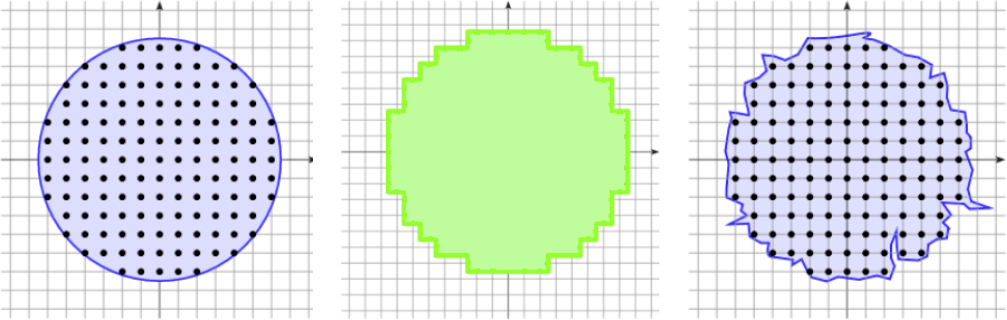
\includegraphics[scale=1]{figures/ambiguity.png}
\caption{\textbf{Digitization ambiguity.} The middle image (in green) is a valid digitization for both the left and right continuous shapes (in blue).}
\label{fig:digitization-ambiguity}
\end{figure}
%
%
\begin{definition}[Multigrid convergence for local geometric quantites]
  A local discrete geometric estimator $\hat{z}$ of some geometric
  quantity $z$ is (uniformly) multigrid convergent for some family $\mathbb{X}$ of Euclidean shapes if
  and only if, for any $X \in \mathbb{X}$, there exists a grid step
  $h_X>0$ such that the estimate $\hat{z}(D(X,h), P,h)$ is
  defined for all $P \in \partial_hX$ with $ 0 < h < h_X$, and
  for any $Q \in \partial X$,
  \begin{equation*}
    \forall P \in  \partial_hX \text{ with } \norm{ P - Q }_{\infty} \leq h, \norm{ \hat{z}(D(X,h),P,h) - z(X,Q)} \leq \tau_{X}(h),			
  \end{equation*}
  where $\tau_{X}:\mathbb{R}^{+}\setminus\{0\} \rightarrow
  \mathbb{R}^{+}$ has null limit at $0$. This function defines the
  speed of convergence of $\hat{z}$ towards $z$ for $X$.
\end{definition}
	
For a global geometric quantity (e.g. perimeter, area, volume), the definition remains the same, except that the mapping
between $\partial X$ and $\partial_h X$ is no longer necessary.

Recently, estimator for curvature and perimeter estimators have been proved multigrid convergent. We propose to use such estimators to estimate the elastica energy of digital shapes
%
%
\begin{align}
	\hat{E}_r\big( D(X,h),h,\alpha,\beta) \big) = \sum_{\vec{e} \in \partial D(X,h)}{ \hat{s}(\vec{e})\left(\; \alpha + \beta \hat{\kappa}_{r}^2(D(X,h),\dot{\vec{e}},h) \; \right)}.
	\label{eq:digital-energy}
\end{align}
%
%
The function $\hat{s}$ denotes the elementary length estimator, i.e., a measure of length is assigned to each edge $\vec{e}$ of digital curve $\partial D(X,h)$. The elementary length is computed using the \emph{$\lambda$-MST} estimator of tangent~\cite{lachaud07tangent,lachaud06hdr}, proven multigrid convergent for the family of convex shapes that are twice differentiable and have continuous curvature. The speed of convergence is $O(h^{1/3})$.

The function $\hat{\kappa} _r$ denotes an estimator of curvature. We use the integral \emph{invariant estimator}~\cite{coeurjolly13integral}, proven multigrid convergent for the family of compact shapes in the plane with $3$-smooth contour. Its convergence speed is of the order of $O(h^{\frac{1}{3}})$ for radii chosen as $r=\Theta (h^{\frac{1}{3}})$~\cite{lachaud2017robust}. We present its definition since it is in the core of the proposed model in this paper.
%
%
\begin{align}
  \tilde{\kappa}_r(D(X,h),P,h) \coloneqq \frac{3}{r^3}\left( \frac{\pi r^2}{2} - \widehat{\text{Area}}\big( D(B_r(P),h) \cap D(X,h),h\big) \right),
  \label{eq:curvature_approximation}
\end{align}
%
%
where the estimation of area for some digital set $S$ can be defined as $\widehat{\text{Area}}(S,h) \coloneqq h^2\text{Card}\left( S \right).$ 

Equation~\ref{eq:curvature_approximation} estimates the curvature as a scaling factor of the difference between the intersection area of a disk of radius $r$ centered at point $P$ of the contour with half of the disk area. Therefore, we can say that the curvature is lower at points in which the balance between intersected and non intersected points is closer to zero.

In the following, we simply write $S$ to specify a digital shape and we omit the grid step $h$ to simplify expressions (or, putting it differently, we assume that the shape of interest is rescaled by $1/h$ and we set $h = 1$).


\section{Balance coeficient and curve-shortening flow}
%
%
\begin{figure}
 \center
 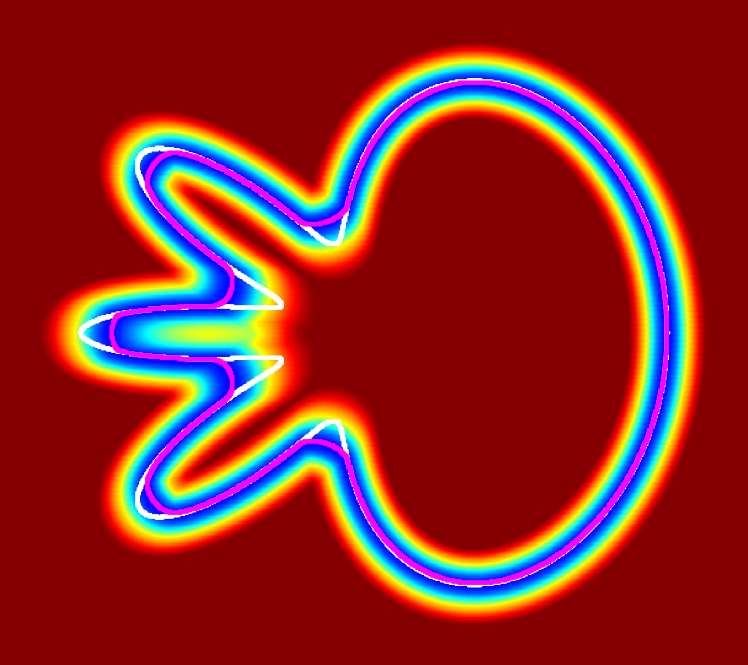
\includegraphics[scale=0.32]{figures/zero-level-set/balance-coefficient-zero-level-set.png}
 \caption{\textbf{Balance coefficient zero-level set}. Evolving the initial contour (colored in white) to the zero-level set of the balance coefficient (colored in black) is closeley related with the curve-shortening flow.}
 \label{fig:balance-coefficient-zero-level-set}
 \end{figure}
%
%
Let $X \subset \R^2$ be an Euclidean shape, $r$ a positive real number and $P$ an arbitrary point of $\R^2$. We define the \emph{balance coefficient $u_r$} of $X$ at $P$ as
%
%
\begin{align*}
  u_r(X,P) &= \left( \frac{\pi r^2}{2} - \text{Area}(B_r(P) \cap X) \right).
\end{align*}
%
%
We observe that the balance coefficient definition is similar to the
integral invariant estimator of curvature in
equation~\eqref{eq:curvature_approximation} (we can model the
continuous domain as a digital domain with an infinitely small grid
step). However, we do not use it to estimate the curvature, but rather
as an indicator of the degree of convexity of the shape.

In the following, we use the balance coefficient to define the balance
coeficient flow and we show how it relates with the curve-shortening
flow (CSF), the one-dimensional version of the mean curvature flow.

\begin{definition}[Balance coefficient flow]
  Let $X \subset \Omega$ be a Euclidean shape and $r>0$ the radius of the disk used to compute the balance coefficient. We define the \emph{balance coefficient flow} for discrete time steps as the sequence of Euclidean shapes
%
%
\begin{align}
  X^{(0)} & := X, \nonumber \\
  \forall k \in \Z, k > 0, \quad X^{(k+1)} & := \left\{ x \in \Omega \: | \: u_r(X^{(k)}, x) \leq 0 \right\}. \label{eq-balance-coefficient-flow}
\end{align}
%
%
\end{definition}
%
%
 One iteration of the balance coefficient flow applied on shape $X$ is equivalent to find the shape $X'$ such that for any disk of radius $r$ centered at any point of the contour of $X'$, the intersection of the disk with the shape $X$ equals $\pi r^2/2$. This interpretation is illustrated in Figure~\ref{fig:geometric-interpretation}.
%
% 
\begin{figure}
\center
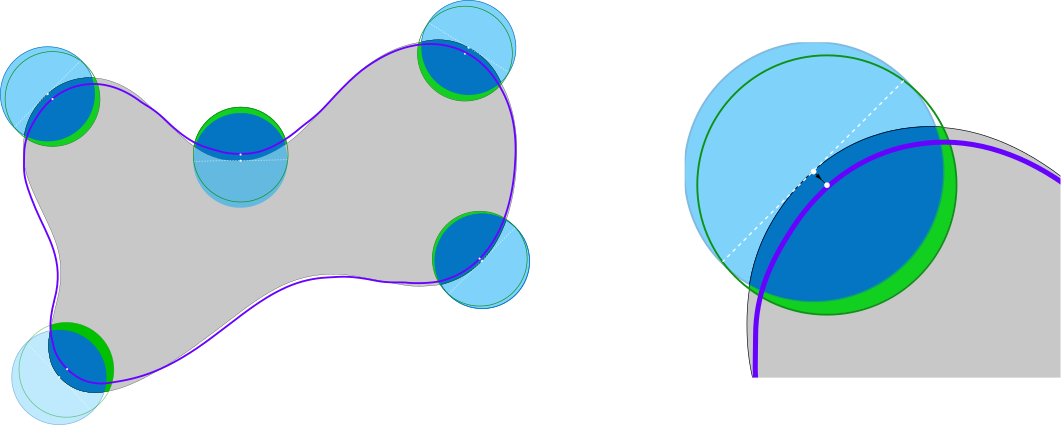
\includegraphics[scale=0.25]{figures/zero-level-set/geometric-interpretation.png}
\caption{\textbf{Geometric interpretation of the balance coefficient flow.} A single iteration of the balance coefficient flow evolves the shape $X$ to the shape $X'$ such that any disk of radius $r$ centered at any point of the contour of $X'$ intersects  an area of $\pi r^2/2$ of the initial shape $X$.}
\label{fig:geometric-interpretation}
\end{figure}
% 
%

Let us show the link between the balance coefficient flow and the
curve-shortening flow. First we rewrite the balance coefficient flow
as a contour evolution. Let us denote $C^{(0)} := \partial
X^{(0)}$ the boundary of $X^{(0)}$. Then, for $x \in C^{(0)}$,
let $\epsilon^{(0)}(x)$ be a solution to the equation
\begin{align} \label{eq-null-balance-coefficient}
  u_r(X^{(0)}, x +\epsilon^{(0)}(x)
  \mathbf{n}^{(0)}(x)) & = 0, \\
  |\epsilon^{(0)}(x)| & < r, \nonumber
\end{align}
with $\mathbf{n}^{(0)}(x)$ the outward normal vector at $x$ to
the boundary of the shape $X^{(0)}$. Specifying
$|\epsilon^{(0)}(x)| < r$ clearly imposes a unique solution to
\Equ{eq-null-balance-coefficient}, provided $r < 1/\kappa$. Then the
contour evolution of $C^{(0)}$ is defined as:
\begin{align} \label{eq-balance-coefficient-contour-flow}
  C^{(1)} := \left\{ \sigma^{(0)}(x), x \in C^{(0)} \right\},
\end{align}
where $\sigma^{(0)}$ is the mapping from $C^{(0)}$ to $C^{(1)}$, such that $x$ maps to $x+\epsilon^{(0)}(x) \mathbf{n}^{(0)}(x)$.

The following proposition indicates that $C^{(1)}$ coincides with
the boundary of $X^{(1)}$ under some hypotheses.

\begin{proposition} \label{prop-C-equ-X}
  If $r$ is small enough, the boundaries of shapes $X^{(0)}$ and
  $X^{(1)}$ are Jordan curves, and the boundary of shape $X^{(0)}$ is
  twice differentiable, then $C^{(1)}$ is the boundary of $X^{(1)}$,
  and the mapping $\sigma^{(0)}$ between $C^{(0)}$ and $C^{(1)}$ is
  bijective.
\end{proposition}
\begin{proof}
  By definition, the curve $C^{(0)}$ is the boundary of shape
  $X^{(0)}$. 
  Being twice differentiable the curve $C^{(0)}$ has a reach that is
  greater than some $\rho > 0$. Hence, any point at distance lower
  than $\rho$ from $C^{(0)}$ has a unique closest point on this
  curve, in the direction normal to the curve.

  Let $x$ be a point on $C^{(1)}$ and let
  $y=\sigma^{(0)}(x)=x+\epsilon^{(0)}(x) \mathbf{n}^{(0)}(x)$.
  Obviously, the smaller is $r$, the closer is $C^{(1)}$ from
  $C^{(0)}$.  From the definition of balance coefficient, one can see
  that the displacement that is solution to
  \Equ{eq-null-balance-coefficient} cannot exceed $\frac{1}{2}\kappa
  r^2$. So if $r < \sqrt{2\rho / \kappa_{\max}}$, where
  $\kappa_{\max}$ is the maximum absolute curvature of the curve, then
  the point $y$ is within the reach of the curve $C^{(0)}$. It follows
  that the mapping $\sigma^{(0)}$ is bijective. It is also continuous
  since all functions are continuous (the area of the shape
  intersected by a ball is continuous with respect to a displacement
  of the ball center).  Hence $C^{(1)}$ is a Jordan curve within the
  reach of $C^{(0)}$. It has therefore an interior component $I$.

  It is clear also that $y \in X^{(1)}$ since $u_r(X^{(0)},y)=0$.
  Let us denote $z(\lambda)=(1-\lambda)x+\lambda y$.

  If $u_r(X^{(0)},x)<0$ then $u_r(X^{(0)},z(\lambda))$ is by
  construction strictly increasing for increasing values of $0 \le
  \lambda \le 1+\nu$, $\nu \ll 1$, and so becomes positive for
  $1<\lambda < 1 + \nu$. In this case $C^{(0)}$ was concave at $x$,
  so the straight segment $\lbrack x,y \rbrack$ is included in
  $X^{(1)}$ and $y$ lies on its boundary. We have also $X^{(1)}
  \cap \lbrack x,y \rbrack \subset I$, and $x$ lies in the interior of
  $X^{(1)}$.
  
  If $u_r(X^{(0)},x)>0$ then $u_r(X^{(0)},z(\lambda))$ is by
  construction strictly decreasing for increasing values of $0 \le
  \lambda \le 1+\nu$, $\nu \ll 1$, and so becomes negative for
  $1<\lambda < 1 + \nu$.  In this case $C^{(0)}$ was convex at $x$,
  so the straight segment $\lbrack x,y \lbrack$ is excluded from
  $X^{(1)}$ and $y$ lies on its boundary. We have also $X^{(1)}
  \cap \lbrack x(1),x(1+\nu) \rbrack \subset I$ and $x(1+\nu)$ lies in
  the interior of $X^{(1)}$.

  In both case we can see that $y$ lies on the boundary of
  $X^{(1)}$. So $C^{(1)} \subset \partial X^{(1)}$. Since both
  are Jordan curves they must coincide and $C^{(1)} = \partial
  X^{(1)}$.  Finally, the interior of $X^{(1)}$ must coincide with
  $I$ since both are finite, they share the same boundary, and they
  share points (whether the boundary is convexe or concave).
  \qed
\end{proof}

The proof tells us that the radius $r$ must be smaller that
$\min(\sqrt{2\rho / \kappa_{\max}},2 / \kappa_{\max})$, for $\rho>0$
smaller than the reach of the shape and $\kappa_{\max}$ the maximal
absolute curvature of the shape.

Let us recall that the curve-shortening flow for a small time step
$t>0$, may be defined as:
\begin{align}
  \Gamma^{(0)} & := \partial X \nonumber \\
  \Gamma^{(t)} & := \left\{ x + t\kappa(x)\mathbf{n}(x), x \in \Gamma^{(0)} \right\}, \label{eq-csf}
\end{align}
denoting by $\kappa(x)$ the curvature of the curve at point $x$
and by $\mathbf{n}(x)$ the outward normal vector at $x$.

Of course, there are implicitly defined variants of this formulation
that allows topology changes, but we will restrict ourselves here to
proving the similarity between the balance coefficient flow and the
curve-shortening flow when there is no topology change.


%
\begin{figure}
\center
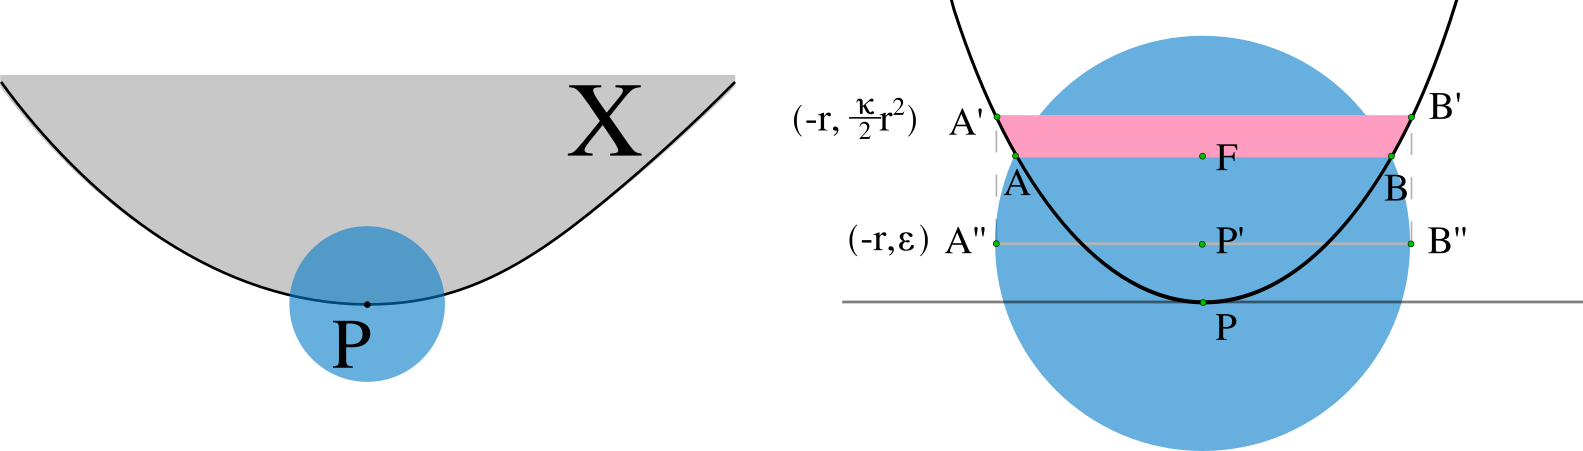
\includegraphics[scale=0.75]{figures/analysis-error/geometry-argument.png}
\caption{\textbf{Balance coefficient and curve-shortening flow (CSF).} We approximate the contour $\partial X$ at $P$ by a parabola. Next, we compute the point $P'$ such that the balance coefficient equals to zero. Our approximation produces an error $\Delta$, highlighted in red, that is of order $O(r^4)$. \label{fig:geometric-argument}}
\end{figure}
%

\begin{proposition}\label{prop:bcf-close-to-csf}
  For small enough $r$, setting $t = \frac{1}{6}r^2$, assuming $C^{(0)}=\Gamma^{(0)}$ is a twice differentiable Jordan curve, then the Hausdorff distance between
  $C^{(1)}$ and $\Gamma^{(t)}$ is some $O(t^2)$, more precisely we get:
  \begin{align*}
    d_H( C^{(1)}, \Gamma^{(t)} ) \le \frac{3}{4} \kappa_{\max}^3 t^2.
  \end{align*}
\end{proposition}
\begin{proof}
  Let $y \in C^{(1)}$. According to Proposition~\ref{prop-C-equ-X},
  there is a point $P \in C^{(0)}$ such that
  $y=\sigma^{(0)}(x)$. Finally, let $y'=P+t\kappa(P)\mathbf{n}(P)$. We
  will show that $\| y-y' \| \le \frac{3}{4} \kappa_{\max}^3 t^2$,
  which induces the result (we could have chosen $y'$ first, and
  obtain the same $y$).

  We center the reference frame on $P$ with $y$-axis aligned with the
  normal vector $\mathbf{n}(P)$.  Since $r$ is small enough, the
  contour is well approximated by the parabola $f(x) :=
  \frac{\kappa(P)}{2}x^2$ in this frame.

  We know that $y = P + \epsilon^{(0)}(P)\mathbf{n}(P)$ according
  to \Equ{eq-null-balance-coefficient}, where $\epsilon^{(0)}(P)$ is
  the local displacement of $P$ which induce a zero balance
  coefficient. Let us determine this displacement $\varepsilon :=
  \epsilon^{(0)}(P)$ in the normal direction, such that the
  intersection of the disk with $X$ equals half of the disk area. Let
  us say that the point of zero balance coefficient is $P'$ and that
  $A_{\varepsilon}$ is the intersection area of the displaced
  disk (see Figure~\ref{fig:geometric-argument}, right, for notations). Then,
%
%
\begin{align*}
	 & A_{\varepsilon} = \frac{\pi r ^2}{2} 
	 && \Leftrightarrow & 2r\varepsilon = \int_{-r}^{r}{\frac{1}{2}\kappa x^2dx} \pm \Delta 
	&& \Leftrightarrow & & \varepsilon = \frac{1}{6}\kappa r^2 \pm \frac{\Delta}{2r}.
\end{align*}
%
%
It remains to compute an upper bound for the error $\Delta$. Let $A^3$ be the leftmost intersection point between the line $A'B'$ and the estimation disk. It is clear that $\Delta/2$ is smaller than the region between $A''A'A^3$ and the arc going from $A^3$ to $A''$. Let $d$ be the length of the segment $A'A''$. 
%
%
\begin{align*}
	Area(A''A'A^3) &= \int_0^d{r - \sqrt{r^2 - x^2} dx} \\
				   &= -\frac{r^2}{2}sin^{-1}\left(\frac{d}{r}\right) + dr - \frac{d}{2}\sqrt{r^2-d^2} \\
				   &\approx \frac{d^3}{6r}.
\end{align*}
%
%
In general, $d$ is bounded by $\frac{1}{2}\kappa r^2$, hence it follows:
%
%
\begin{align*}
	\frac{\Delta}{2} \leq \frac{d^3}{6r} \leq \frac{1}{48}\kappa^3r^5.
\end{align*}
%
%
Therefore,
%
%
\begin{align*}
	\varepsilon &= \frac{1}{6}\kappa r^2 \pm \frac{1}{48}\kappa^3r^4.
\end{align*}
%
%
To conclude the argument, we have:
\begin{align*}
  \| y - y' \| & = \| P + \epsilon^{(0)}(P)\mathbf{n}(P) - (P+t\kappa(P)\mathbf{n}(P)) \| \\
  & = | \varepsilon - t \kappa(P) | \\
  & \le \left| \frac{1}{6}\kappa(P) r^2 - t\kappa(P) \right| + \frac{1}{48}|\kappa|^3r^4\\
  & \le \frac{1}{48}|\kappa(P)|^3r^4 && \text{(since $t=\frac{1}{6}r^2$)} \\
  & \le \frac{3}{4}\kappa_{\max}^3 t^2 && \text{(since $|\kappa(P)| \le \kappa_{\max}$)}
\end{align*}
\mbox{~}\hfill\qed
\end{proof}

Applying Proposition~\ref{prop-C-equ-X} at each time step $k$ (writing
$(k)$ instead of $(0)$ and $(k+1)$ instead of $(1)$) allows us to
redefine the balance coefficient flow as the sequence $C^{(k)}$,
provided that the boundaries of $X^{(k)}$ are twice differentiable
Jordan curves. But Proposition~\ref{prop:bcf-close-to-csf} applied on
these consecutive curves tells us that the curves $C^{(k)}=\partial
X^{(k)}$ are very close to the curve shortening flow, which induces
twice differentiable curves except at critical points. Proving that
the flow $X^{(k)}$ also mimicks the curve-shortening flow across
critical points would require much more mathematical work and is
outside the scope of this paper.

%% %
%% \begin{proposition}\label{prop:balance-coefficient-curve-shortening-flow}
%% Let $X$ an Euclidean shape such that the contour of $X$, denoted $\partial X$, is twice differentiable. Then, there is an injective map between the contours of two consecutive shapes in the balance coefficient flow
%% %
%% %
%% \begin{align*}
%% 	\sigma^{(t)} &: \partial X^{(t)} \rightarrow \partial X^{(t+1)} \\	
%%     \sigma^{(t)}(P) &= P + \varepsilon(p)N^{(t)}(P),
%% \end{align*}
%% %
%% %
%% where $\varepsilon(P)=\frac{1}{6}\kappa(P)r^2 + O(r^4)$ and $N^{(t)}(P)$ the normal vector at $\partial X^{(t)}(P)$.
%% \end{proposition}
%% %
%% %
%% \begin{proof}
%% 	Let $P$ a point in the contour of $X$ where we initially center the estimation disk of radius $r$. We assume that the contour of $X$ at point $P$ has locally a curvature of $\kappa$ and that $r \ll 1/\kappa$. Therefore, the contour is well approximated by the parabola $f(x) := \frac{\kappa}{2}x^2$ in the frame centered on $P$ and oriented toward inside $X$ in the direction of the normal vector. 
	
%% 	 The goal is to find the displacement $\varepsilon$ of center $P$ in the normal direction such that the intersection of the disk with $X$ equals half of the disk area. Let us say that the point of zero balance coefficient is $P'$ and that $A_{\varepsilon}$ is the intersection area of the displaced disk. Then,
%% %
%% %
%% \[
%% \begin{array}{>{\displaystyle}r>{\displaystyle}r>{\displaystyle}l}
%% 	& A_{\varepsilon} &= \frac{\pi r ^2}{2} \\[1em] 
%% 	\Leftrightarrow & 2r\varepsilon &= \int_{-r}^{r}{\frac{1}{2}\kappa x^2dx} \pm \Delta \\[1em]
%% 	\Leftrightarrow & \varepsilon &= \frac{1}{6}\kappa r^2 \pm \frac{\Delta}{2r}.
%% \end{array}
%% \]
%% %
%% %
%% We proceed by computing an upper bound of the error $\Delta$. Let $A^3$ be the leftmost intersection point between the line $A'B'$ and the estimation disk. It is clear that $\Delta/2$ is smaller than the region between $A''A'A^3$ and the arc going from $A^3$ to $A''$. Let $d$ be the length of the segment $A'A''$. 
%% %
%% %
%% \begin{align*}
%% 	Area(A''A'A^3) &= \int_0^d{r - \sqrt{r^2 - x^2} dx} \\
%% 				   &= -\frac{r^2}{2}sin^{-1}\left(\frac{d}{r}\right) + dr - \frac{d}{2}\sqrt{r^2-d^2} \\
%% 				   &\approx \frac{d^3}{6r}.
%% \end{align*}
%% %
%% %
%% In general, $d$ is bounded by $\frac{1}{2}\kappa r^2$, hence it follows:
%% %
%% %
%% \begin{align*}
%% 	\frac{\Delta}{2} \leq \frac{d^3}{6r} \leq \frac{1}{48}\kappa^3r^5.
%% \end{align*}
%% %
%% %
%% Therefore,
%% %
%% %
%% \begin{align*}
%% 	\varepsilon &= \frac{1}{6}\kappa r^2 \pm \frac{1}{48}\kappa^3r^4.
%% \end{align*}
%% %
%% %
%% \qed
%% \end{proof}
%% %
%% %
%% Proposition~\ref{prop:balance-coefficient-curve-shortening-flow} states that, if the radius of the estimation disk is sufficiently small, then the balance coefficient flow behaves similar to the curve-shortening flow. In other words,
%% %
%% %
%% \begin{corollary}
%% Given the conditions of proposition~\ref{prop:balance-coefficient-curve-shortening-flow}, and for a sufficiently small value of $r$, the balance coefficient flow can be written as
%% %
%% %
%% \begin{align*}
%% 	\frac{ d}{dt} \partial X &= \kappa N.
%% \end{align*}
%% %
%% %
%% \end{corollary}
%% %
%% %
%% \begin{proof}
%% We set
%% \begin{align*}
%% 	\Delta t(r,\kappa) &= \frac{1}{6}r^2 \pm \frac{1}{48}\kappa^2r^4.
%% \end{align*}
%% We choose $r$ such that $r \ll \kappa(P)$ for all $P$ in $\partial X$. Then,
%% %
%% %
%% \begin{align*}
%% 	\partial X^{(t+1)} - \partial X^{(t)} &= \varepsilon(P)N^{(t)}(P) \\
%% 	&= \kappa(P)N^{(t)}\Delta t(r,\kappa). 
%% \end{align*}
%% %
%% %
%% Rearranging the terms we obtain
%% %
%% %
%% \begin{align*}
%% 	\frac{\partial X^{(t+1)} - \partial X^{(t)}}{\Delta t(r,\kappa)} &= \kappa(P)N^{(t)}
%% \end{align*}
%% %
%% %
%% Finally, taking the limit as $r \rightarrow 0$
%% %
%% %
%% \begin{align*}
%% 	\frac{d}{dt}\partial X &= \kappa N. 
%% \end{align*}
%% %
%% %
%% \qed
%% \end{proof}
%
%
The CSF has many interesting properties~\cite{huisken84flow,gage86heat,ecker2008heat}. Among those, the CSF is the continuous deformation that decreases the perimeter of a single closed curve at the fastest speed; and it also preserves convexity. In particular, the CSF eventually collapses the initial curve to a single point.

There are interesting links between the CSF and a variant of the heat equation defined for the indicatrix function of a set~\cite{merriman1992diffusion}. In this same work, the authors informally give a geometric interpretation for the CSF that is equivalent to our zero-level set of the balance coefficient. A technique that emerged from the interpretation of CSF as a heat equation is the so called threshold dynamics~\cite{esedoglu2005threshold,esedoglu2008threshold}. However, the use of threshold dynamics for image processing tasks is not immediate due to the difficulty to inject a data fidelity term. That is not the case in our approach.

We are going to apply the balance coefficient flow in a discrete setting. In theory, that means that we have some limitations regarding the choice of the estimation radius $r$, the grid resolution $h$ and the real curvature value at the estimation point. In general, we need to respect
%
%
\begin{align*}
	h \ll r \ll \frac{1}{\kappa}.
\end{align*}
%
%
In practice, we are going to show that we can achieve good results without being too strict regarding the restriction above.
%
%
\section{Elastica minimization of digital shapes via graph cuts}
We recall our estimator for the elastica energy 
%
\begin{align}
	\hat{E}_{\Theta}\big( S \big) = \sum_{\vec{e} \in \partial S}{ \hat{s}(\vec{e})\left(\; \alpha + \beta \hat{\kappa}_{r}^2(S,\dot{\vec{e}}) \; \right)}.
	\label{eq:elastica-estimator-2}
\end{align}
%
%
Notice that we group all parameters in vector $\vec{\Theta}=(h,r,\alpha,\beta)$. We remark that, since it is composed of multigrid convergent estimators, the elastica estimator is also multigrid convergent~\cite{lachaud06hdr}.

In this section we describe a graph-cut model for the optimization of digital shapes with respect the elastica energy.

 
\subsection{Graph cut model}\label{sec:graph-cut-model}

We are going to evolve the initial contour $\partial S$ of some digital shape $S$ to the zero-level set of its balance coeficient by computing the minimum cut of some directed graph. Since the balance coefficient is a local quantity, it is sufficient to define the graph in a band around the initial contour.

Let $d_{S}:\Omega \rightarrow \mathbb{R}$ be the signed Euclidean distance transformation with respect to shape $S$. The value $d_{S}(P)$ gives the Euclidean distance between $P \notin S$ and the closest point in $S$. For points $P \in S$, $d_{S}(P)$ gives the negative of the distance between $P$ and the closest point not in $S$.

\begin{definition}[Optimization band]
Let $S \subset \Omega \subset \mathbb{Z}^2$ a digital set and natural number $n>0$. The optimization band $O_n(S)$ is defined as
%
%
\begin{align*}
	O_n(S) &:=\left\{ P \in \Omega \; | \; -n \leq d_{S}(P) \leq n \right\}.
\end{align*}
\end{definition}
%
%
\begin{definition}[Candidate graph]
Let $S \subset \Omega \subset \mathbb{Z}^2$ a digital set and natural number $n>0$. We define $\mathcal{G}(n,S,\mathcal{V},\mathcal{E})$ as the candidate graph of $S$ with optimization band $n$ such that
%
%
\begin{align*}
\mathcal{V} &= \big\{\; v_P \; | \; P \in O_n(S) \;\} \cup \{s,t \big\}, \\
\mathcal{E} &= \mathcal{E}_u \cup \mathcal{E}_{st}, \\
\mathcal{E}_u &= \big\{ \; \{v_P,v_Q\} \; | \; P \in O_n(S) \text{ and } Q \in \mathcal{N}_4(P) \; \big\}, \\
\mathcal{E}_{st} &= \big\{\; \{s,v_P\} \; | \; d_S(P)=-n \; \big\} \cup \big\{\; \{v_P,t\} \; | \; d_S(P)=n \; \big\}.
\end{align*}
%
%
\end{definition}

The vertices $s,t$ are virtual vertices representing the source and target vertices as it is usual in a minimum cut framework. We denote $\mathcal{N}_4(P)$ the set of $4$-adjacent neighbors of $P$. The innermost (outermost) pixels of the optimization band are connected to the source (target), and we identify such vertices as
%
%
\begin{align*}
	\mathcal{V}_s &:=\left\{ v_P \in \Omega \; | \; d_{S}(P) = -n \right\}, \\
	\mathcal{V}_t &:=\left\{ v_P \in \Omega \; | \; d_{S}(P) = n \right\}.
\end{align*}
%
%
The set $\mathcal{E}_{st}$ comprises all the edges having the source as their starting point or the target as their endpoint. In table~\ref{tab:edge-capacity} we describe the edge capacity function.
%
%
\begin{table}
\begin{center}
\begin{tabular}{|c|c|c|}
\hline
\textbf{edge} $e$ & $\mathbf{c(e)}$ & \textbf{for}\\
\hline
$\{v_P, v_Q\}$ & $ \frac{1}{2}\left( u_r(S,P) + u_r(S,Q) \right) $ & $\{v_P,v_Q\} \in \mathcal{E}_{u}$\\
\hline
$\{v_P, s\}$ & $M$ & $v_P \in \mathcal{V}_{s}$ \\
\hline
$\{v_P, t\}$ & $M$ & $v_P \in \mathcal{V}_{t}$ \\
\hline
\end{tabular}
\end{center}
,where $M$ is defined such that
%\begin{align*}
%	M &= 1+\max_{p \in O_n(S)} 2*u(S,h,r,p).
%\end{align*}
\begin{align*}
	M &= \max_{e \in \mathcal{E} }{ c(e) }.
\end{align*}
\caption{\textbf{Edge capacity function.}}
\label{tab:edge-capacity}
\end{table}
%
%

A cut in a graph separates the vertices in source and target components. Our model is defined such that the source component of the minimum cut gives the next shape in the iteration. In other words, let $mincut(\mathcal{G})$ denote the source component of the minimum cut of capacitated graph $\mathcal{G}$. Then, we define
%
%
\begin{align}
	\forall t \geq0, \quad S^{(t+1)} = mincut\left( \mathcal{G}(S^{(t)}) \right), 
	\label{eq:no-neighborhood-process}
\end{align}
%
%
where $S^{(0)}$ is the initial shape. Here and in the following, we omit some parameters of the candidate graph to simplify notation. They are going to be explicitly defined if necessary.

In figure~\ref{fig:no-neighborhood-shapes-evolution}, we show some examples of this process. As expected, the flow is very similar to the CSF. Next, we describe how to optimize the shape with respect the elastica energy by using a neighborhood of shapes.
%
%
%
\begin{figure}
	\center
	\subfloat[\label{}]{%
	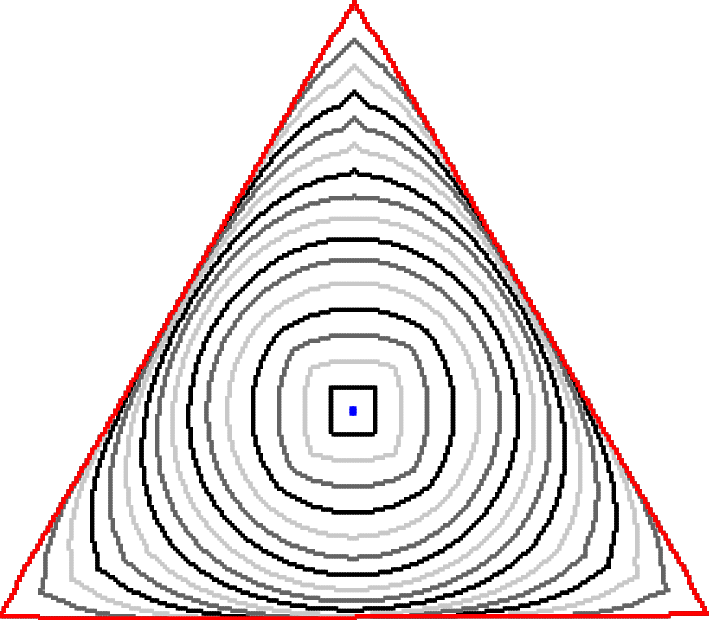
\includegraphics[scale=0.12]{figures/no-neighborhood-flow/triangle.png}}\hspace{2em}%
	\subfloat[\label{}]{%
	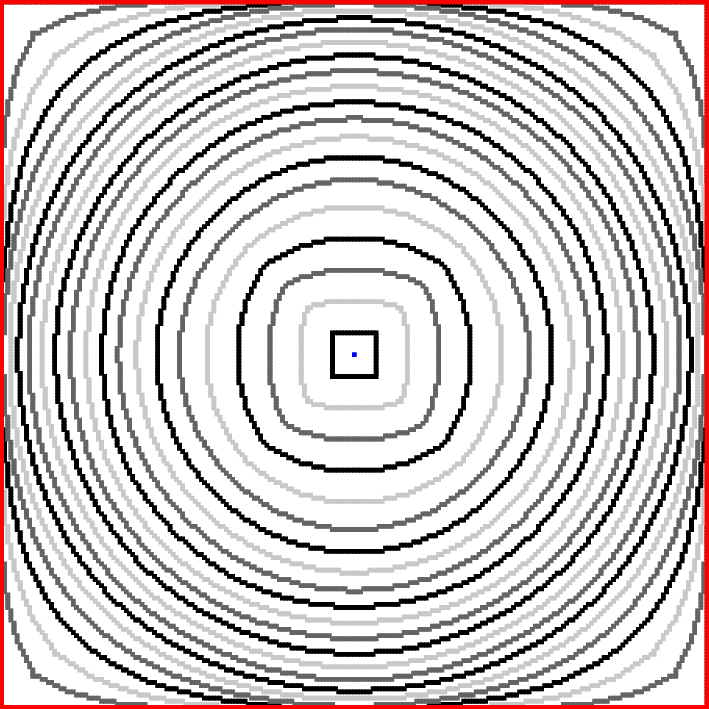
\includegraphics[scale=0.11]{figures/no-neighborhood-flow/square.png}}\hspace{2em}%	
	\subfloat[\label{}]{%
	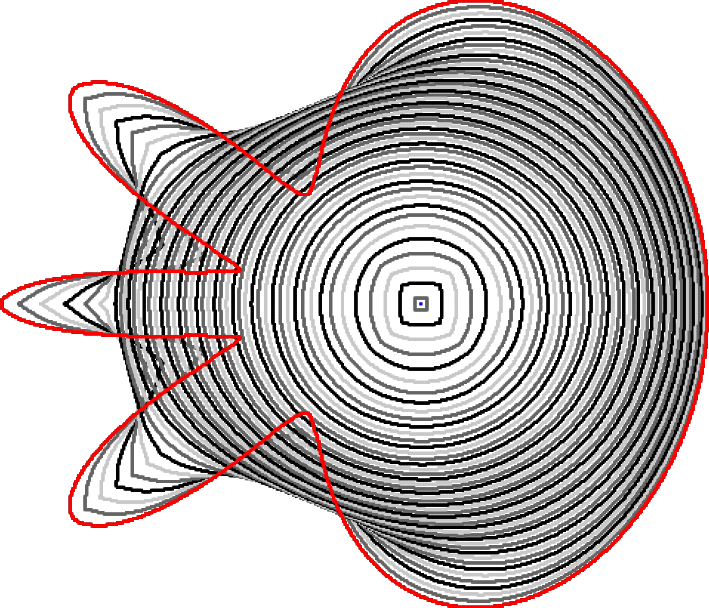
\includegraphics[scale=0.14]{figures/no-neighborhood-flow/flower.png}}	
	\caption{\textbf{No neighborhood of shapes}. Evolution with no neighborhood of shapes defined $(h=1/8,r=2)$. The evolution miicks the curve-shortening flow. Initial contour is colored in red and each other contour is ploted every 10 iterations.}
	\label{fig:no-neighborhood-shapes-evolution}
\end{figure}
%
%
%
%\begin{figure}
%	\center
%	\subfloat[\label{}]{%
%	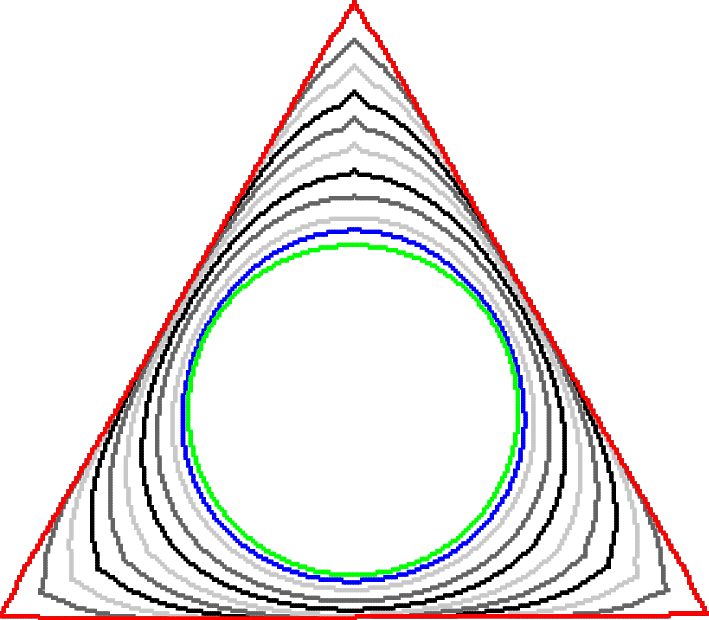
\includegraphics[scale=0.12]{figures/no-neighborhood-flow-improve-always/triangle.png}}\hspace{2em}%
%	\subfloat[\label{}]{%
%	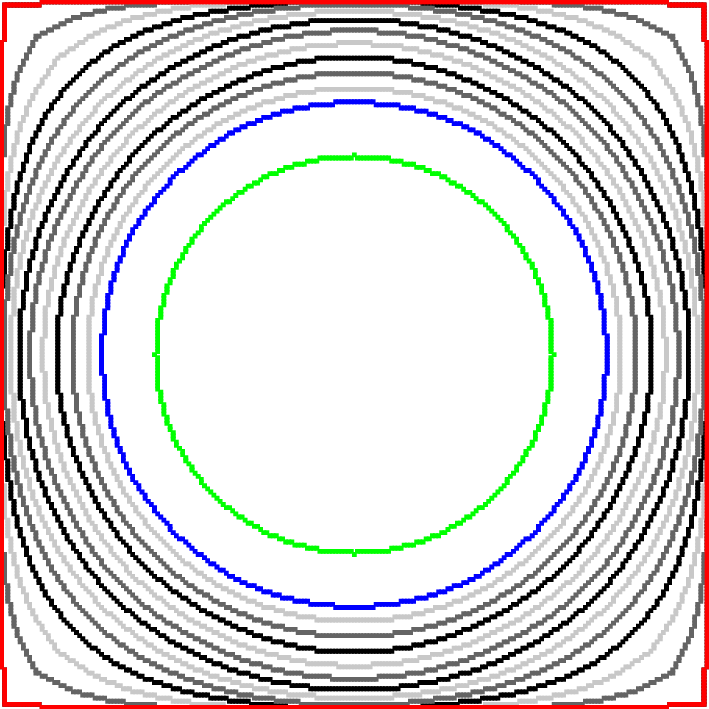
\includegraphics[scale=0.11]{figures/no-neighborhood-flow-improve-always/square.png}}\hspace{2em}%	
%	\subfloat[\label{}]{%
%	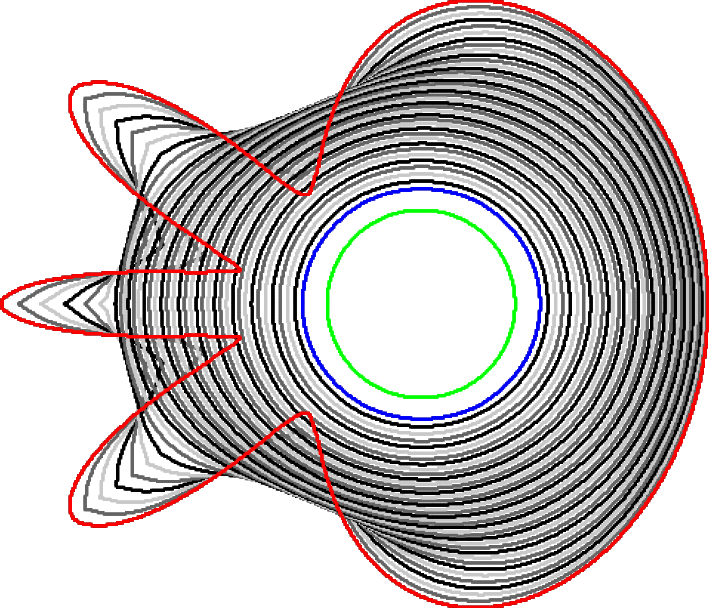
\includegraphics[scale=0.14]{figures/no-neighborhood-flow-improve-always/flower.png}}	
%	\caption{\textbf{Stop if elastica increases}. In red the initial contour and in blue the final contour given by the evolution process with no neighborhood of shapes $\vec{\Theta} = (h=1/8,r=2,\alpha=1/64,\beta=1)$. The optimum contour is highlighted in green (a disk of radius $8$). Intermediate contours are ploted every 10 iterations.}
%	\label{fig:no-neighborhood-shapes-evolution-improve-always}
%\end{figure}

\subsection{Neighborhood of shapes}

We are going to show how the process~\ref{eq:no-neighborhood-process} can be modified to optimize the elastica energy. We start by defining a very simple neighborhood of shapes.
%
%
\begin{definition}[Neighborhood of shapes]
	Let $S$ a digital shape. We define its neighborhood $\mathcal{N}(S)$ as the set
	\begin{align*}
		\mathcal{N}(S) &= \Big\{S, S^{+1},S^{-1} \big\},
	\end{align*}
	where $S^{+1}$ ($S^{-1}$) denotes a morphologic dilation (erosion) by a square of side $1$.
\end{definition}
%
%
The Graph Flow Algorithm (GFA)~\ref{alg:graphflow-algorithm} summarizes the process and figure~\ref{fig:graph-flow-experiments} show some experiments.
%
%
\begin{algorithm}
 \SetKwData{It}{t}
 \SetKwData{MIt}{maxIt}
 \SetKwData{Delta}{delta}
 \SetKwInOut{Input}{input}\SetKwInOut{Output}{output}
 \SetKwComment{comment}{//}{}
 
 \Input{A digital set $S$; the optimization band $n$; parameter vector $\vec{\theta}=(h,r,\alpha,\beta)$; the maximum number of iterations \MIt;} 
 \BlankLine
 $S^{(0)} \longleftarrow S$\; 
 \BlankLine
 $t \longleftarrow 0$\;
 \While{ \It $<$ \MIt  }{ 	
	\comment{Candidate selection} 
	$\mathcal{C}^{(t)} \longleftarrow \bigcup_{S' \in \mathcal{N}(S^{(t)})} \Big\{ mincut(\mathcal{G}(S') \Big\}$ \;

	\BlankLine
	\comment{Candidate validation}
	$S^{(t+1)} \longleftarrow \displaystyle \argmin_{ S' \in \mathcal{C}^{(t)} }{ \hat{E}_{\vec{\theta}}(S')}$\; 	
	\It $\longleftarrow$ \It $+1$\;
	
 }
 \caption{Graph Flow Algorithm (GFA).}
 \label{alg:graphflow-algorithm}  
\end{algorithm}

\begin{figure}
\begin{minipage}{0.25\textwidth}
\center
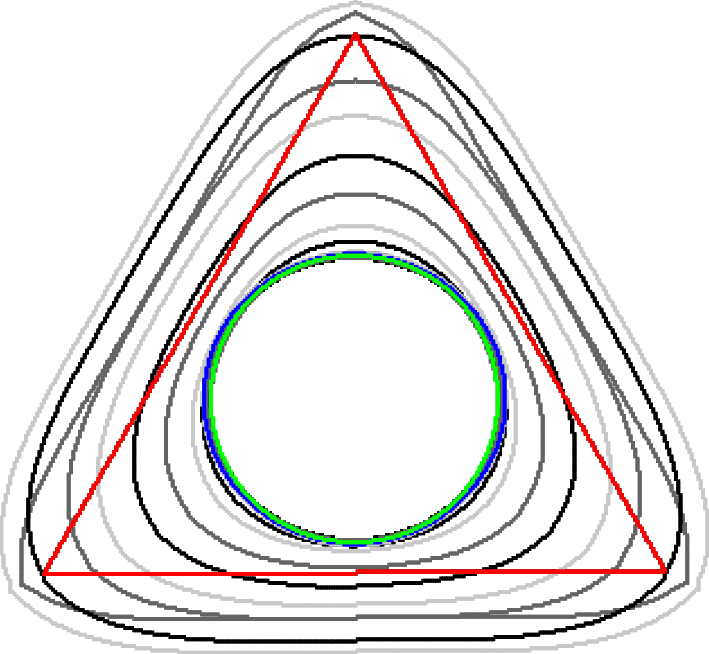
\includegraphics[scale=0.10]{figures/shape-flow/summaries-r8/triangle.png}

\vspace{1.5em}

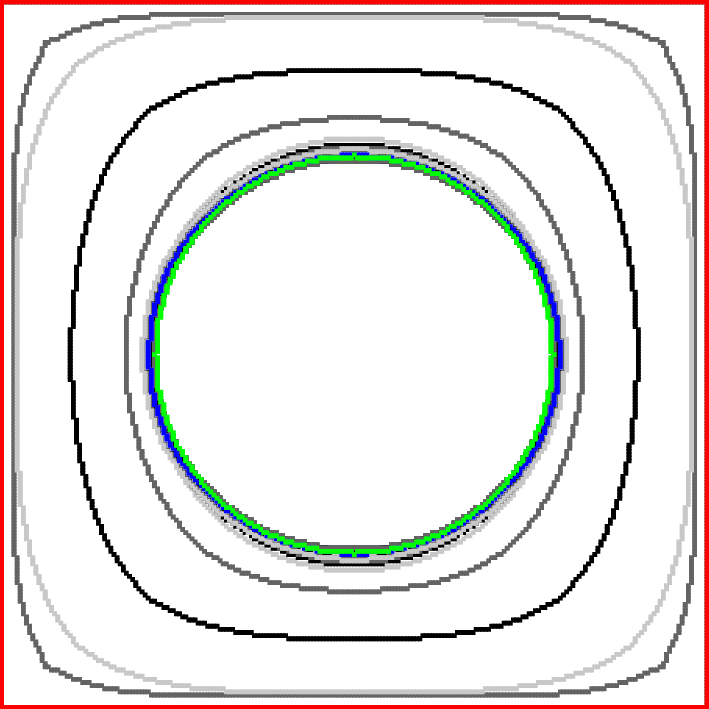
\includegraphics[scale=0.08]{figures/shape-flow/summaries-r8/square.png}

\vspace{1.5em}

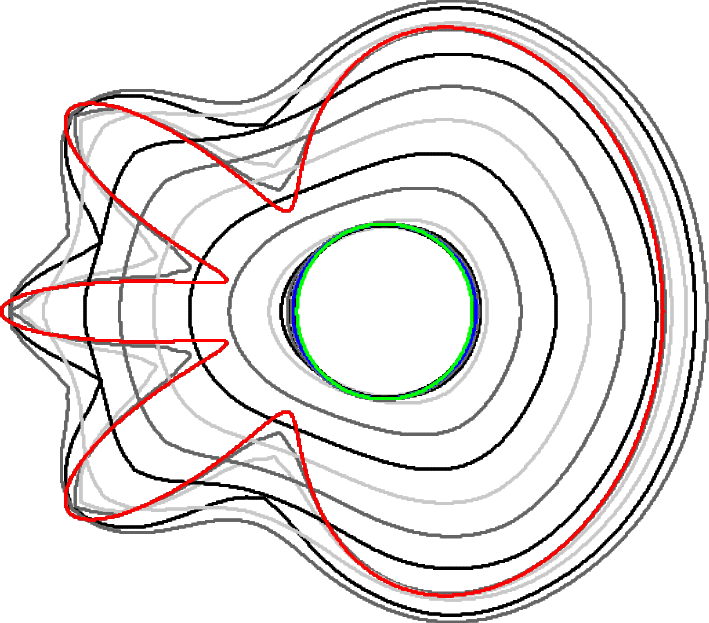
\includegraphics[scale=0.10]{figures/shape-flow/summaries-r8/flower.png}

\vspace{1.5em}

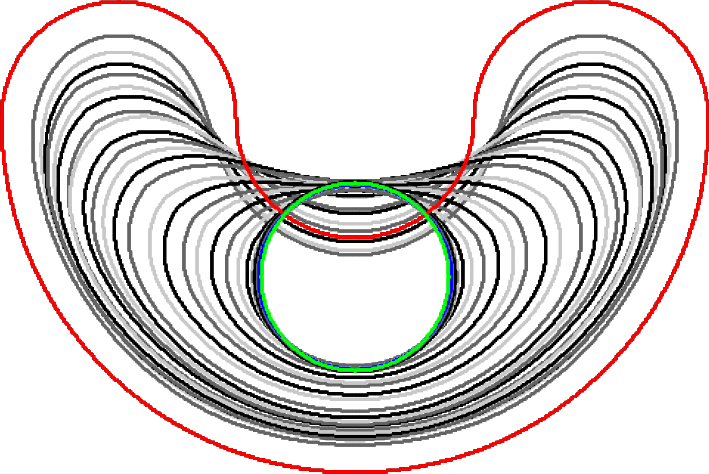
\includegraphics[scale=0.10]{figures/shape-flow/summaries-r8/bean.png}
\end{minipage}%
\begin{minipage}{0.75\textwidth}
\center
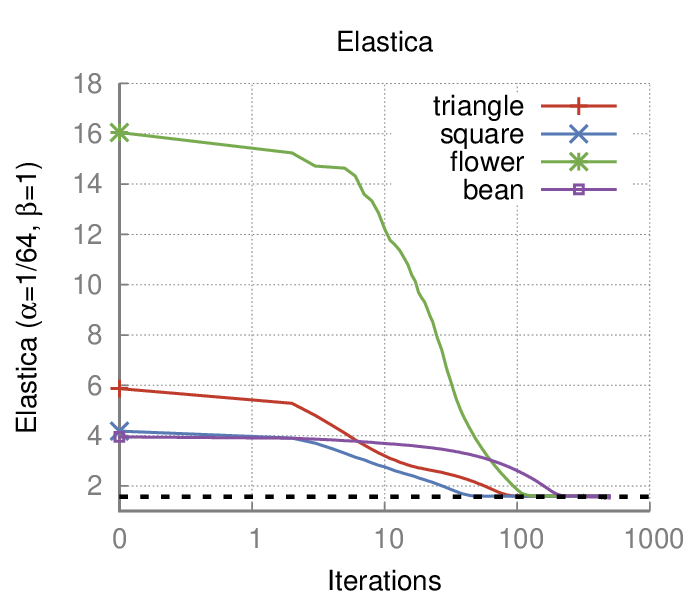
\includegraphics[scale=0.22]{figures/shape-flow/plots/elastica.png}

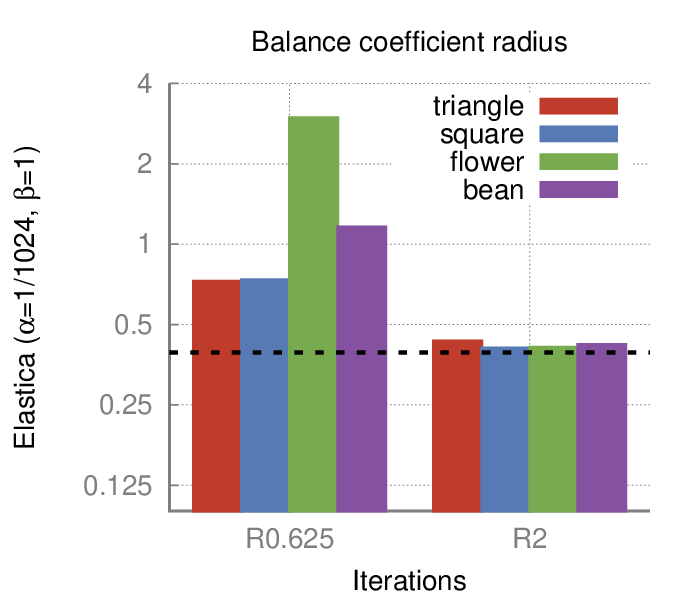
\includegraphics[scale=0.22]{figures/shape-flow/plots/bars.png}
\end{minipage}
\caption{\textbf{GFA experiments}. In the left, the evolution of various shapes given by the GFA $(h=1/8,r=2)$. The red and blue contours highlight initial and final contours. The green contour is the optimum solution. The top right graph describes the reduction in elastica energy. The dotted line marks the optimum energy value (a disk of radius $8$). The bottom right graph points out the importance of a right choice of the balance coefficient radius (the optimum solution in this case is a disk of radius 32).}
\label{fig:graph-flow-experiments}
\end{figure}

Remarkably, the GFA escapes premature local minimum and even achieves the global optimum of the elastica energy for some cases. In figure~\ref{fig:graph-flow-expand} we show the results of elastica minimization for $\vec{\Theta} = ( r=2,h=1/8,\alpha=1/1024,\beta=1 )$. The GFA correctly expands the shapes to the optimum disk of radius $32$. However, we may have a premature interruption of the evolution if a small estimation disk radius is chosen, as illustrated in the bottom right graph of figure~\ref{fig:graph-flow-experiments}.
%
%
\begin{figure}
\center
\subfloat[]{
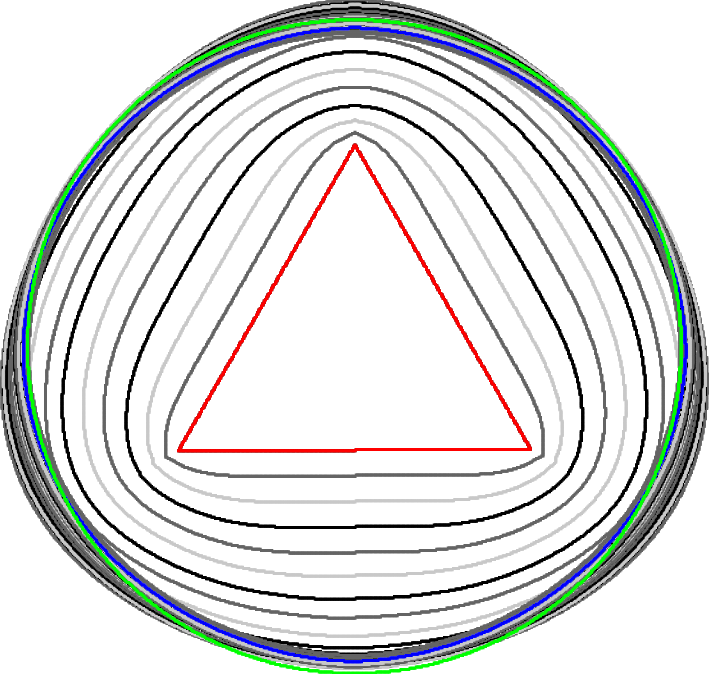
\includegraphics[scale=0.13]{figures/shape-flow/summaries-r32/triangle.png}}\hspace{1.5em}%
\subfloat[]{
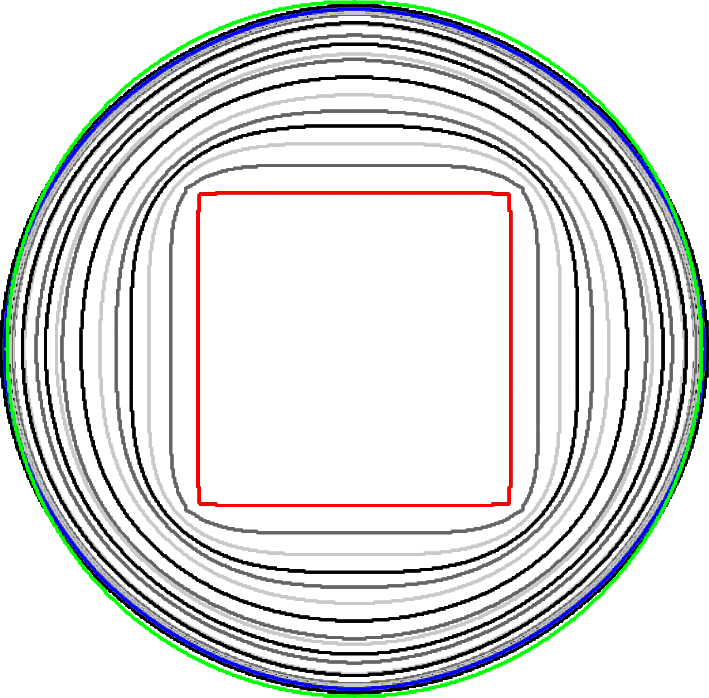
\includegraphics[scale=0.13]{figures/shape-flow/summaries-r32/square.png}}\hspace{1.5em}%
\subfloat[]{
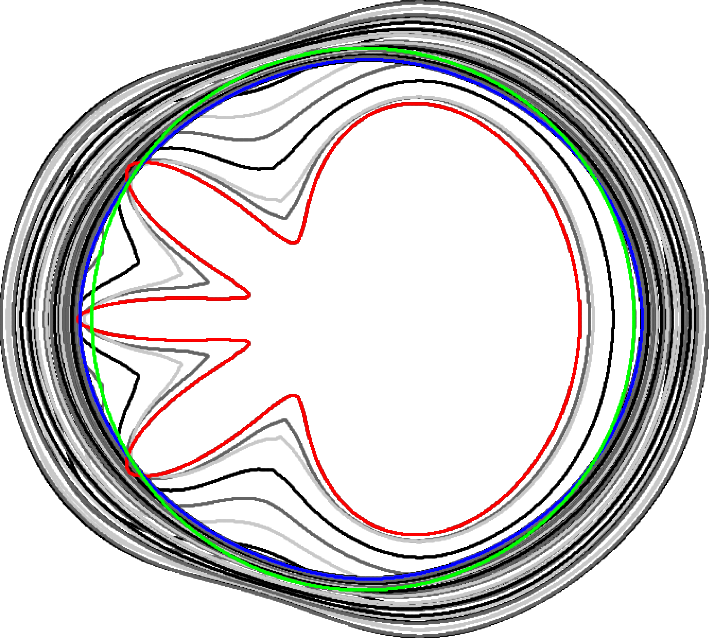
\includegraphics[scale=0.15]{figures/shape-flow/summaries-r32/flower.png}}
\caption{\textbf{GFA can expand the initial shape}. Shapes evolutions by GFA with $\vec{\Theta}(h=1/8,r=2,\alpha=1/1024, \beta=1)$ as the elastica estimator parameters. The green contour highlights the optimum shape (a disk of radius $32$).}
\label{fig:graph-flow-expand}
\end{figure}
%
%
The computations can be done in parallel for each member of the neighborhood. Table~\ref{tab:summary-graph-flow-running-time} shows the running times where the candidate graphs are evaluated in parallel. These times can be further improved by parallelizing the computation of the balance coefficient as well the elastica estimator evaluation.
%
%
\begin{figure}[h!]
\center
\captionsetup{type=table}
\footnotesize
\begin{tabular}{|l|c|c|c|c|}
\hline
& Pixels & It & Time & Time/It\\
\hline
Triangle & 33256 & 120 & 49.6s & 0.4s \\
Square & 51259 & 60 & 24.6s & 0.4s \\
Flower & 119789 & 150 & 132.8s & 0.9s \\
Bean & 100504 & 300 & 148.4s & 0.5s \\
\hline
\end{tabular}
\caption{\textbf{Running time of GFA}. The GFA achieves running times lower than one second per iteration when the shape neighbors are evaluated separately (executed in a Intel Corei7 $1.8GHz$ processor with $16gb$ of ram). There still room for other parallelization and these running times can be further improved.}
\label{tab:summary-graph-flow-running-time} 
\end{figure}
%
%

Finnaly, the GFA is easily modifiable to accomodate image terms, which makes it suitable for image processing tasks. Next, we are going to explore some of these possibilitites in image segmentation.
%
%
\section{Applications in image processing}

The GFA can be extended to include a data fidelity term. In this section, we explore the potential of the GFA to be used in image processing tasks. We present the results of two experiments. The first is targeted to supervised segmentation and the second to unsupervised segmentation. Since we do not have an explicit expression for the input shapes (that is, the objects to segment), the grid resolution is set to $h=1$ in all experiments. The experiments were executed in a Intel Corei7 $1.8GHz$ processor with $16gb$ of ram.


\subsection{Supervised segmentation}

The goal of this experiment is to illustrate the regularization properties of the GFA and to highlight the role of the data term in our approach. The data term employed in this experiment is the same used by Boykov-Jolly in their classical graph cut model~\cite{boykov01graphcut}. 

\subsubsection{Data term}
We are going to update the graph construction described in section~\ref{sec:graph-cut-model} to accomodate the data term. In particular, we define two new sets of vertices $\mathcal{V}_{fg}$ and $\mathcal{V}_{bg}$ as the set of foreground and background seeds, respectively. Those are given as input.

Let $\vec{x} \in \{0,1\}^{|S|}$ represent the label of each pixel in the image ($0$ for background and $1$ for foreground). We define the data term as
%
\begin{align*}
	data(S) &= \gamma_r \sum_{P \in S}{ \psi(x_P) } + \gamma_b \sum_{P \in S}\sum_{Q \in \mathcal{N}_{4}(P)}{\phi_{(P,Q)}},
\end{align*}
where $\gamma_r \geq 0$ and $\gamma_b \geq 0$ are parameters controlling the influence of the regional and boundary terms, respectively. Given the image $I:\Omega \rightarrow [0,1]^3$, the unary and pairwise terms are defined as
\begin{align*}
	\psi(x_P) &= \left\{ \begin{array}{ll}
	-\ln  H_{bg}\big( I(P) \big), & \text{if } x_P=0  \\[1em]	
	-\ln  H_{fg}\big( I(P) \big), & \text{if } x_P=1,
	\end{array}\right.\\[1em]
	\phi_{(P,Q)} &= \left\{ \begin{array}{ll}
	\displaystyle \exp{ \left(- \frac{(I(P) - I(Q))^2}{|P-Q|} \right) }, & Q \in \mathcal{N}_4(P) \\[1em]
	0, & \text{otherwise}.
	\end{array}\right.
\end{align*}
%
The terms $H_{bg}$ and $H_{fg}$ are mixed Gaussian distribution constructed from the foreground and background seeds. The updated capacity function is described in table~\ref{tab:updated-capacity-function}.
%
\begin{table}
\setlength{\extrarowheight}{0.75em}
\begin{center}
\begin{tabular}{|c|c|c|}
\hline
\textbf{edge} $e$ & $\mathbf{c(e)}$ & \textbf{for}\\
\hline
$\{v_P, v_Q\}$ & $\beta \cdot \big(u_r(S,P) + u_r(S,Q)\big) + \gamma_b \cdot \phi_{(P,Q)}$ & $\{v_P,v_Q\} \in \mathcal{E}_{u}$\\
\hline
\multirow{3}{*}{$\{s,v_P\}$} & $\gamma_r \cdot \psi(0)$ & $P \in O_n(S), v_P \notin \mathcal{V}_{fg} \cup \mathcal{V}_{bg}$\\
& $M$ & $v_P \in \mathcal{V}_{s} \cup \mathcal{V}_{fg}$ \\
\hline
\multirow{3}{*}{$\{v_P, t\}$} & $\gamma_r \cdot \psi(1)$ & $P \in O_n(S), v_P \notin \mathcal{V}_{fg} \cup \mathcal{V}_{bg}$ \\
& $M$ & $v_P \in \mathcal{V}_{t} \cup \mathcal{V}_{bg}$  \\
\hline
\end{tabular}
\end{center}
where the constant $M$ is defined such that
\begin{align*}
M &= \max_{e \in \mathcal{E} }{ c(e) }.
\end{align*}
\caption{\textbf{Updated capacity function.} The capacity function of table~\ref{tab:edge-capacity} is updated to accommodate the data term.}
\label{tab:updated-capacity-function}
\end{table}
%
%

To handle bias due to the magnitude difference between data and geometry terms, we normalize them in groups. Regional and boundary terms $\psi,\phi$ are normalized to the interval $[0,1]$ with respect to their values. The same is done, separately, for the curvature term.

To minimize parameter dependence from the image input, we also apply a parameter normalization. Given parameters $\alpha, \gamma_b, \gamma_r$ and an initial segmentation $I_0$, we apply the following normalization factors.
%
\begin{align*}
	\alpha & = \alpha \times 4\pi^2/Per^2 \\
	\gamma_r & = \gamma_r \times \hat{E}(I_0)/data(I_0) \\	
	\gamma_b & = \gamma_b \times \hat{E}(I_0)/data(I_0)		
\end{align*}

That means that by setting $\alpha=\gamma_r=\gamma_b=1$, the shape of minimum elastica is the disk of perimeter $Per$ (assuming no data term); and that $data(I_0)=\hat{E}(I_0)$.
%
%
\subsubsection{Experiment}
We need an initial contour to start the GFA. The initial contour is given by the grabcut algorithm~\cite{rother04grabcut}, a variant of classical graph cut segmentation~\cite{boykov01graphcut} which is implemented in the OpenCV library.

For this experiment, we used a selection of $212$ images of the Validation 2017 subset of the Coco dataset~\cite{lin2014microsoft}. The Coco dataset comprises over $328$k images spreaded over $91$ categories and $11$ super-categories. Table~\ref{tab:image-categories-distribution} summarizes the quantity of selected images per super-category. 
%
%
\begin{table}
\begin{tabular}{cccccc}
\textbf{Person} & \textbf{Vehicle} & \textbf{Food} & \textbf{Animal} & \textbf{Outdoor Obj.} & \textbf{Sports} \\
24 & 22 & 22 & 34 & 16 & 19 \\[1em]
\textbf{Kitchenware} & \textbf{Furniture} & \textbf{Appliance} & \textbf{Electronics} & \textbf{Indoor Obj.} & \\
19 & 17 & 9 & 10 & 19 &
\end{tabular}
\caption{\textbf{Selected images distribution.} The quantity of selected images per Coco super-category. A total of $212$ images were selected.}
\label{tab:image-categories-distribution}
\end{table}
%
%

This experiment consisted in manually select foreground and background seeds for each selected image; compute the grabcut segmentation; and then use the grabcut segmentation as input for two versions of the GFA: one with the data term described in the previous section and another without. In figure~\ref{fig:coco-experiment-sample} we show a sample of the images used in the experiment. All the results are available online and can be conveniently visualized in this webpage~\footnote{https://danoan.github.io/content/papers/coco-experiment/report.html}. 

In table~\ref{tab:coco-experiment-parameter} we list the GFA parameters for this experiment.

\begin{table}
\center
\begin{tabular}{cccc}
\textbf{Estimation radius} & \textbf{Opt. band width} & \textbf{Neighborhood size} & \textbf{Iterations} \\
$\mathbf{(r)}$ & $\mathbf{(n)}$ & $\mathbf{(k)}$ & \textbf{(maxit)}\\
5 & 4 & 3 & 20\\[1em]
\textbf{Length weight} & \textbf{Curvature weight} & \textbf{Boundary weight} & \textbf{Region weight}\\
$\boldsymbol{(\alpha)}$ & $\boldsymbol{(\beta)}$ & $\boldsymbol{(\gamma_b)}$ & $\boldsymbol{(\gamma_r)}$\\
10 & 1 & 1 & 1
\end{tabular}
\caption{\textbf{Supervised experiment parameters}. The list of the GFA parameters for the supervised segmentation experiment.}
\label{tab:coco-experiment-parameter}
\end{table}
%
%
\begin{table}
\center
\begin{tabular}{cccc}
\textbf{Highest} & \textbf{Lowest} & \textbf{Average} & \textbf{Average per iteration} \\
50.3s & 3.3 & 15.1s & 0.7s\\
\end{tabular}
\caption{\textbf{Supervised experiment running time}. The average iteration is of $0.7$s.}
\label{tab:coco-experiment-running-time}
\end{table}
%
%
\begin{figure}
\center
\subfloat[Coco annotations for kite, moto and giraffe]{
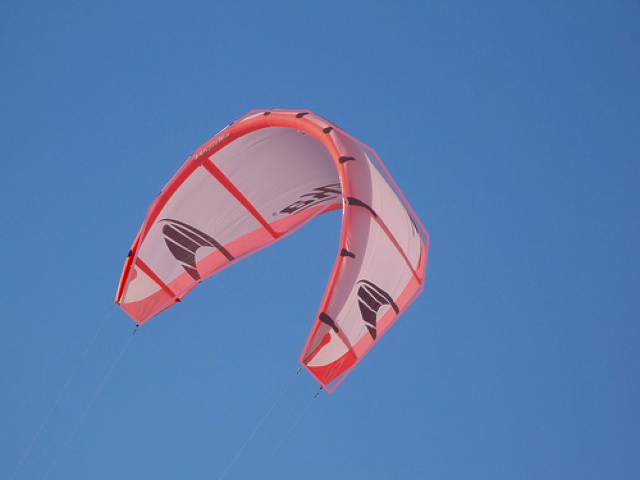
\includegraphics[scale=0.2]{figures/coco-experiment/sample-images/kite/coco-annotation.png}\hspace{1em}
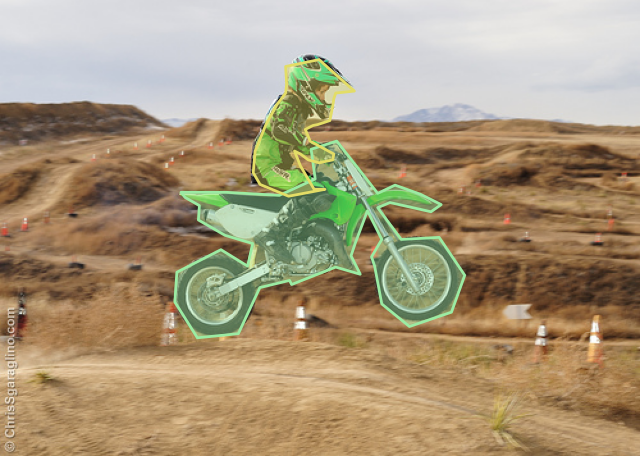
\includegraphics[scale=0.2]{figures/coco-experiment/sample-images/moto/coco-annotation.png}
\hspace{1em}
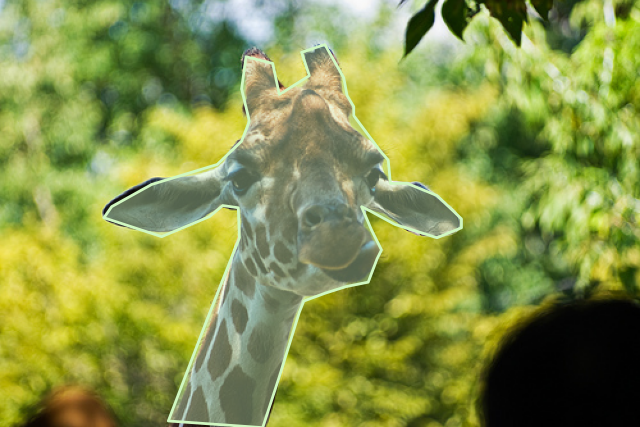
\includegraphics[scale=0.2]{figures/coco-experiment/sample-images/giraffe/coco-annotation.png}
}%

\subfloat[Graph cut segmentation]{
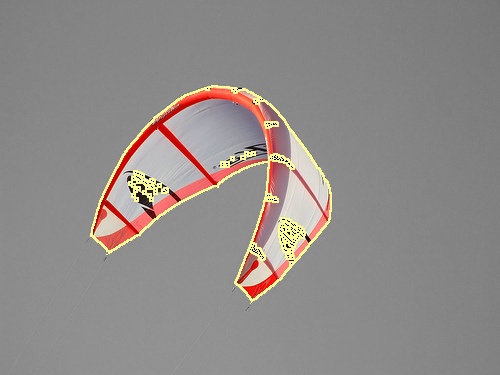
\includegraphics[scale=0.2]{figures/coco-experiment/sample-images/kite/gc-seg.png}
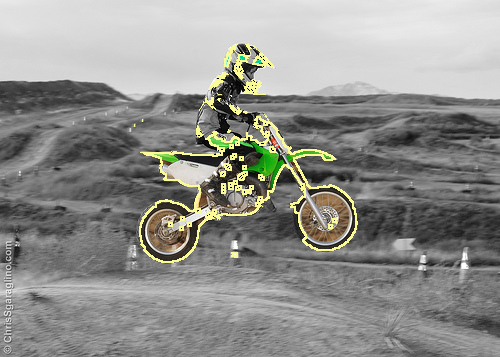
\includegraphics[scale=0.2]{figures/coco-experiment/sample-images/moto/gc-seg.png}
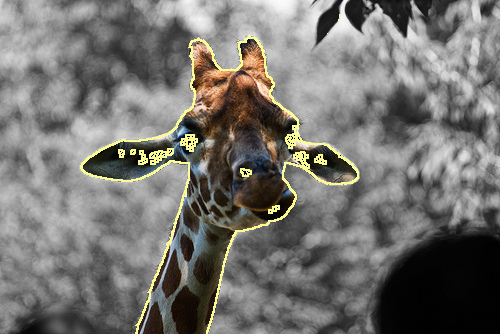
\includegraphics[scale=0.2]{figures/coco-experiment/sample-images/giraffe/gc-seg.png}
}

\subfloat[GFA without data term]{
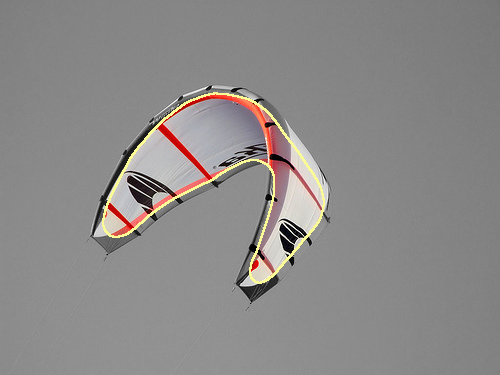
\includegraphics[scale=0.2]{figures/coco-experiment/sample-images/kite/corrected-seg-without-data.png}
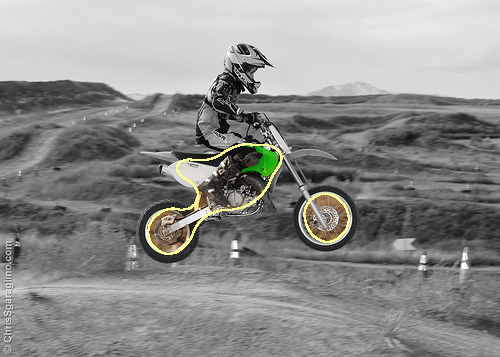
\includegraphics[scale=0.2]{figures/coco-experiment/sample-images/moto/corrected-seg-without-data.png}
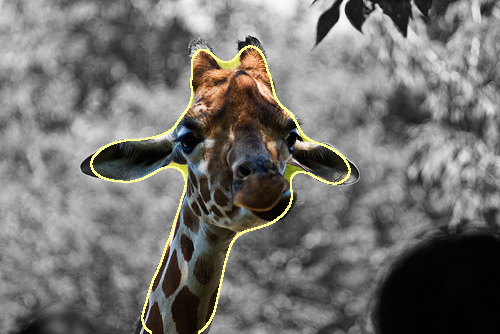
\includegraphics[scale=0.2]{figures/coco-experiment/sample-images/giraffe/corrected-seg-without-data.png}
}

\subfloat[GFA with data term]{
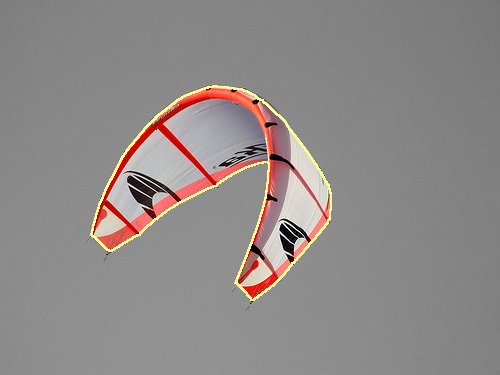
\includegraphics[scale=0.2]{figures/coco-experiment/sample-images/kite/corrected-seg-with-data.png}
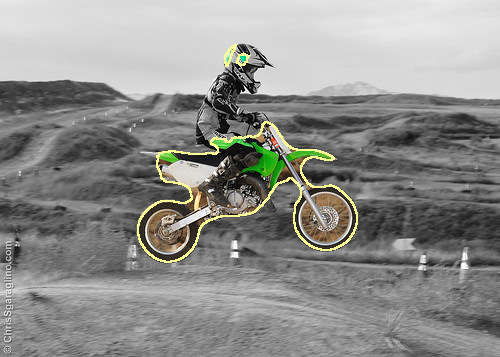
\includegraphics[scale=0.2]{figures/coco-experiment/sample-images/moto/corrected-seg-with-data.png}
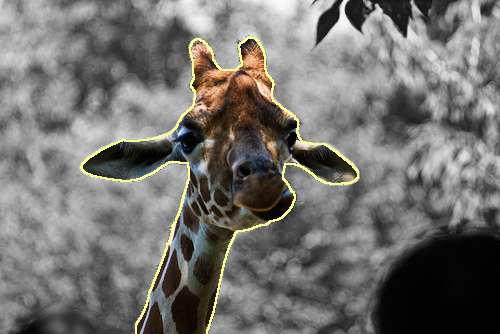
\includegraphics[scale=0.2]{figures/coco-experiment/sample-images/giraffe/corrected-seg-with-data.png}
}
\caption{\textbf{Some results of the supervised segmentation experiment}. Coco annotations are shown in the first line. In the next rows we present the same image segmented by grabcut and corrected by the GFA without and with data term.  }
\label{fig:coco-experiment-sample}
\end{figure}
%
%
%
The first observation is that the GFA regularizes the initial grabcut segmentation contour with respect to the elastica energy. In figure~\ref{fig:coco-tangent-profile} we display the tangent profile of both grabcut segmentation and the one corrected by the GFA. We clearly observe the regularization effect of the GFA with respect the grabcut profile. The value of the elastica energy of the contour and its number of inflection points is also greatly reduced, as it is summarized in figure~\ref{fig:coco-summary-regularization}.

The second observation is that the data term has an important role in the quality of the segmentation with respect to precision and recall metrics, as shown in the box plot of figure~\ref{fig:coco-summary-precision-recall}. That means that by using a model with no data term, such as threshold dynamics, is insufficient to recover segmentations of good quality. In fact, executing the GFA without data term will eventually transform the contour in one or more circles, and we can have an arbitrary bad value for the recall. We can see some of these undesirable effects in the fourth line of figure~\ref{fig:coco-experiment-sample}: the kite area is overly reduced; the motorcycle is separated in two disconnected components; and the giraffe loses part of its ears.

The third observation is that the GFA presents the completion effect that is expected from regularization by the elastica energy. This property is particularly useful for the segmentation of thin and elongated objects, but not only. It also helps to remove oversegmented components which are particularly common in graph cut based models. In figure~\ref{fig:coco-completion} we give some examples of contour completion.

Finally, we remark that all images were executed using the same set of parameters. That is not ideal. Low resolution images should be segmented using a smaller estimation radius, for example. Therefore, all the results presented here could be eventually improved by tuning the parameters accordingly. An example of this is given in figure~\ref{fig:coco-parameter-tuning}.

A summary of the running time is presented in table~\ref{tab:coco-experiment-running-time}. The average running time per iteration is of $0.7$s. We remark that in several cases we need fewer than $5$ iterations to greatly improve regularization metrics such as elastica and inflection points. However, to recover the completion effect we may need more iterations.

%
%
%
%
\begin{figure}
\center
\subfloat[Grabcut segmentation (left) and corrected segmentation by GFA (right).]{
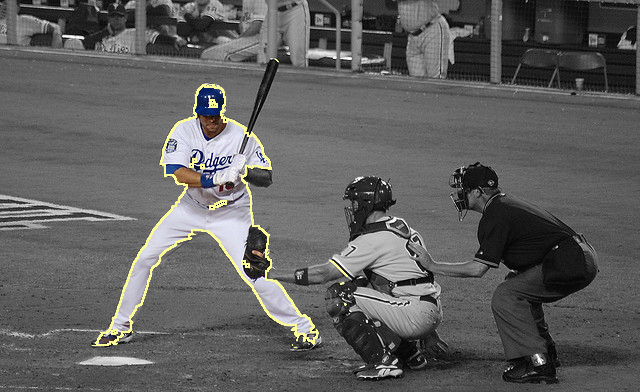
\includegraphics[scale=0.25]{figures/coco-experiment/tangent-profile/baseball/gc-seg.png}\hspace{1em}
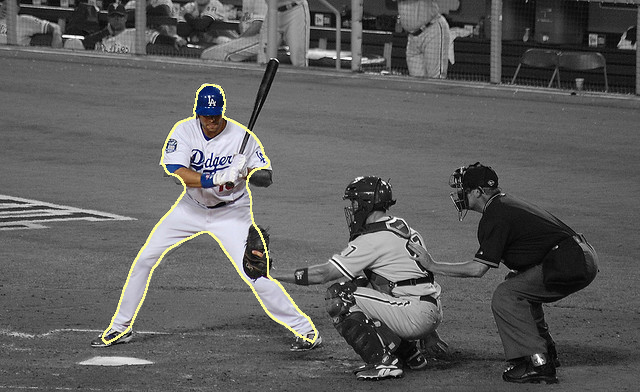
\includegraphics[scale=0.25]{figures/coco-experiment/tangent-profile/baseball/corrected-seg-with-data.png}
}

\subfloat[Tangent profile for grabcut (left) and GFA (right) segmentations.]{
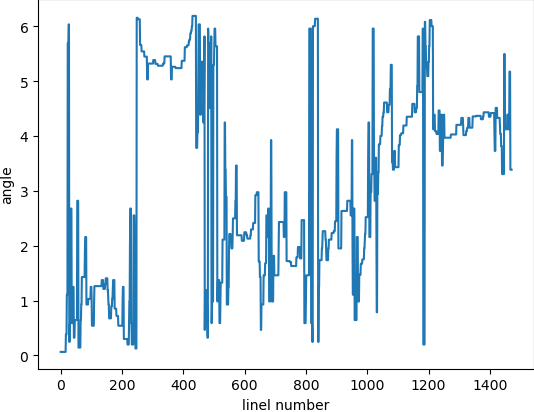
\includegraphics[scale=0.42]{figures/coco-experiment/tangent-profile/baseball/tangent-profile-gc.png}\hspace{1em}
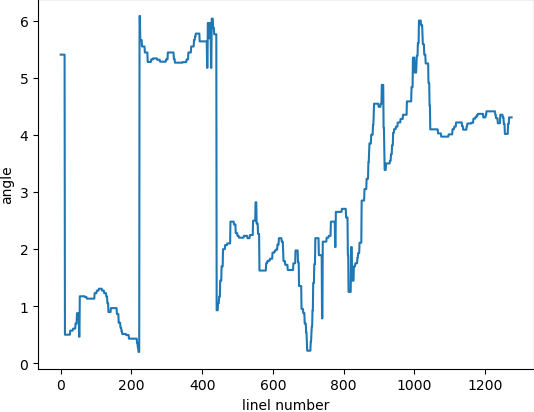
\includegraphics[scale=0.42]{figures/coco-experiment/tangent-profile/baseball/tangent-profile-cc.png}
}
\caption{\textbf{Contour regularization.} The GFA normlalizes the contour with respect the elastica energy. This is illustrated by the tangent profile of the grabcut segmentation and the one corrected by GFA.}
\label{fig:coco-tangent-profile}
\end{figure}
%
%
\begin{figure}
\center
\subfloat[Recall and precision results with respect to Coco annotations.\label{fig:coco-summary-precision-recall} ]{
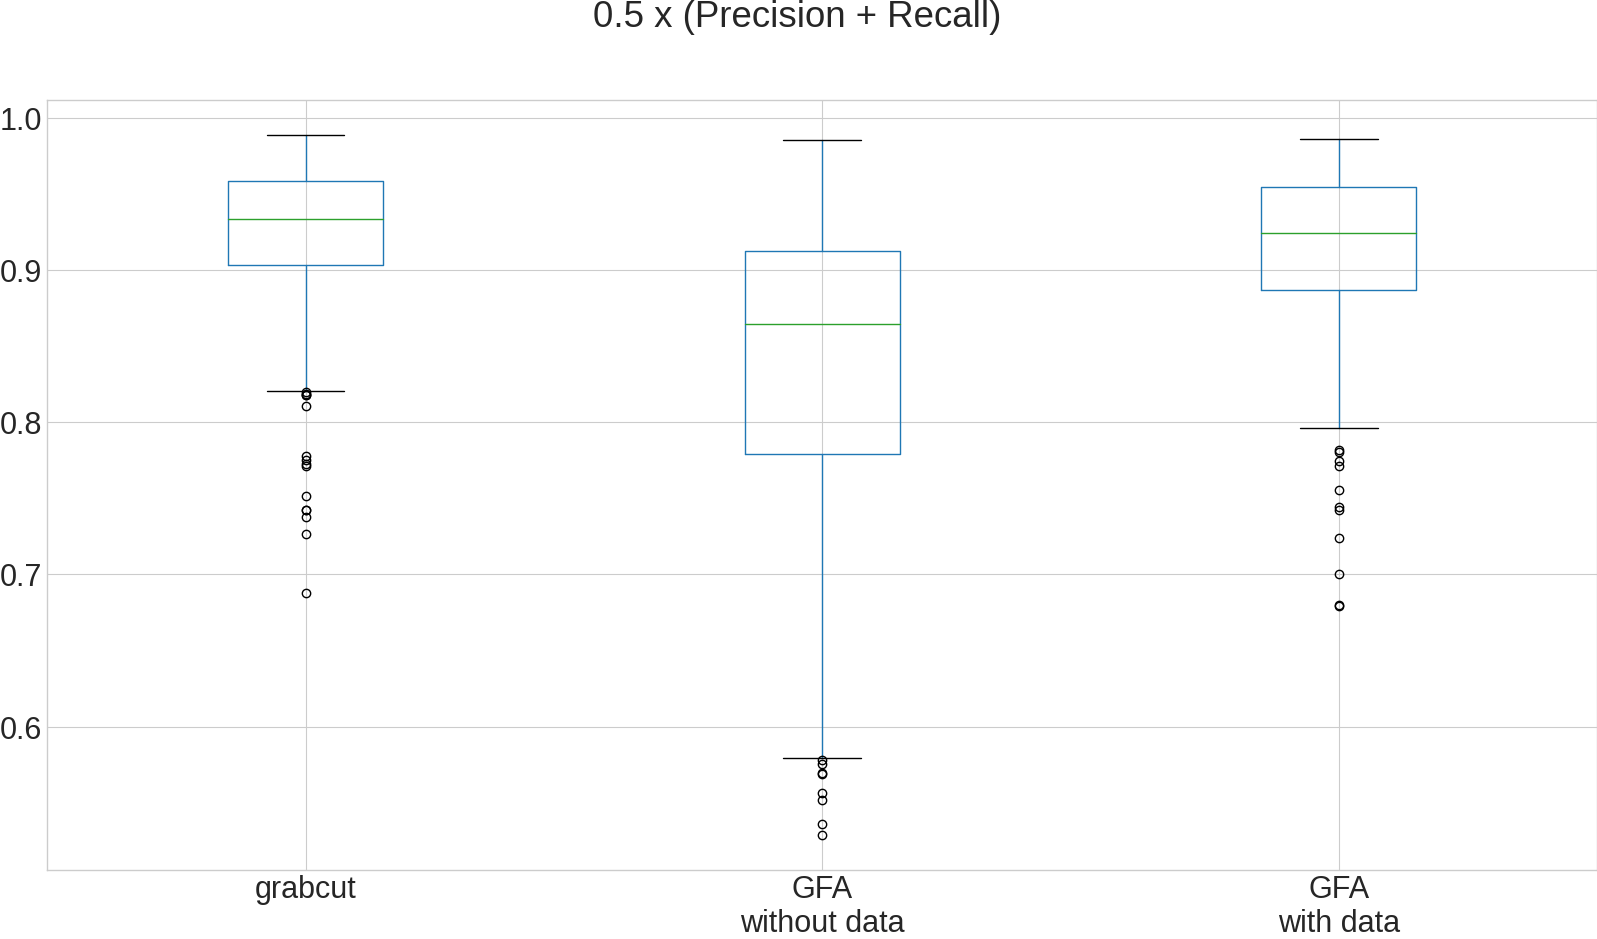
\includegraphics[scale=0.25]{figures/coco-experiment/box-plot-mixed.png}
}

\subfloat[Contour regularization metrics for GFA with respect grabcut.\label{fig:coco-summary-regularization}]{
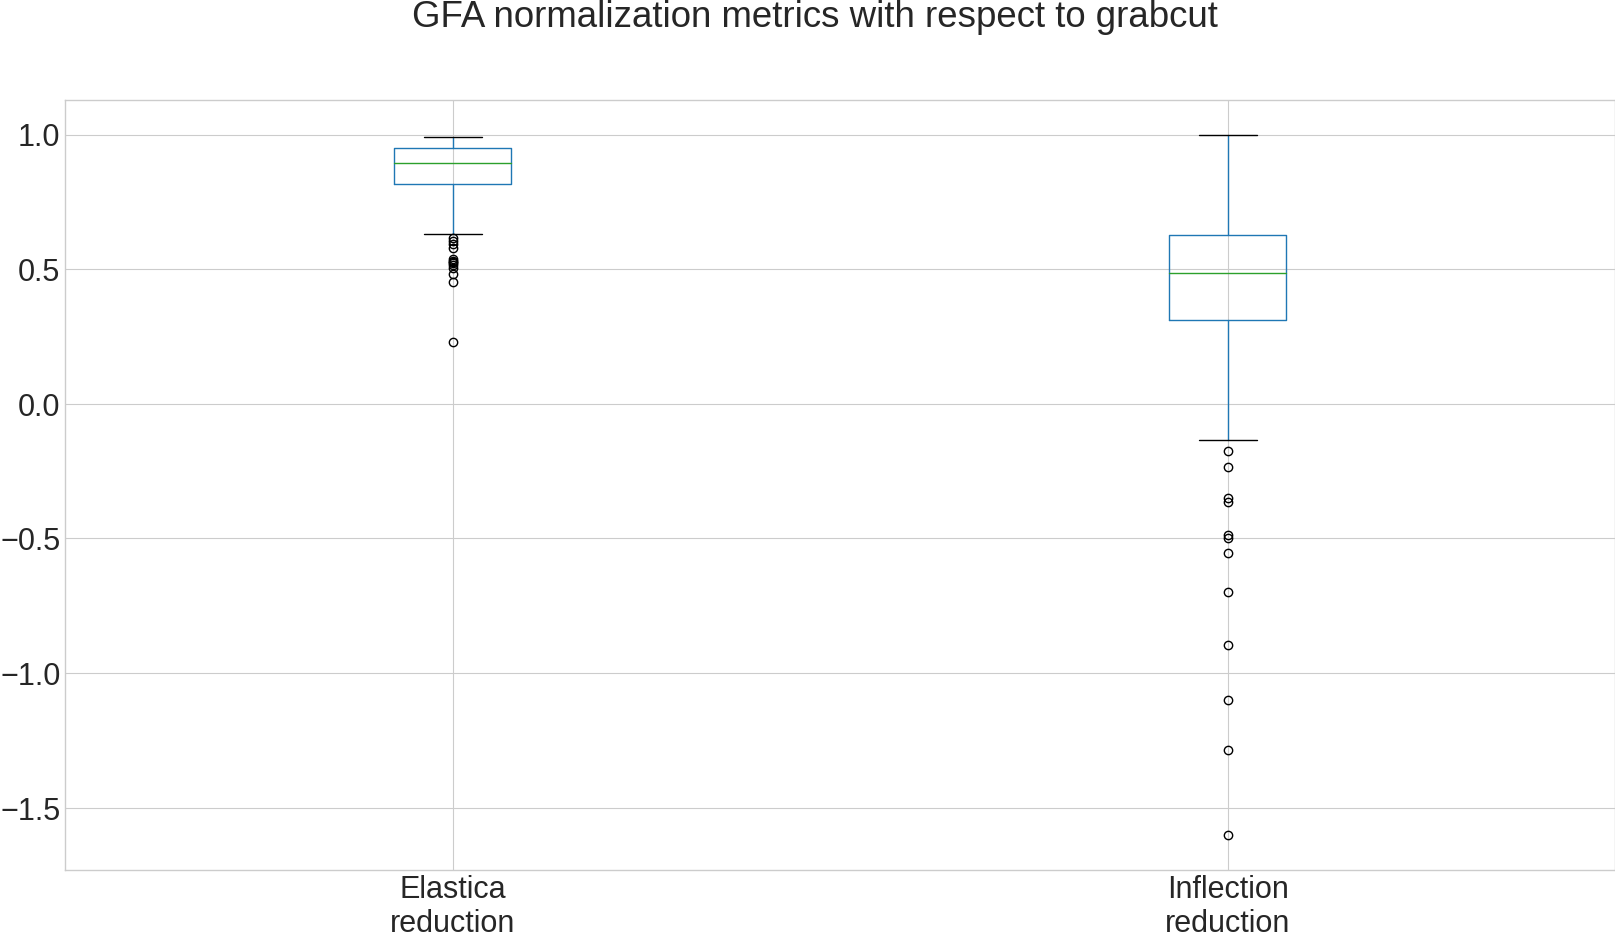
\includegraphics[scale=0.25]{figures/coco-experiment/box-plot-correction.png}
}

\caption{\textbf{Summary statistics.} The GFA give results as good as grabcut with respect to precision and recall, but with a much simpler and easy to describe (and to store) contour.}
\end{figure}
%
%
\begin{figure}
\center
\subfloat[Using $r=5$ ($(P+R)/2=0.78$)]{
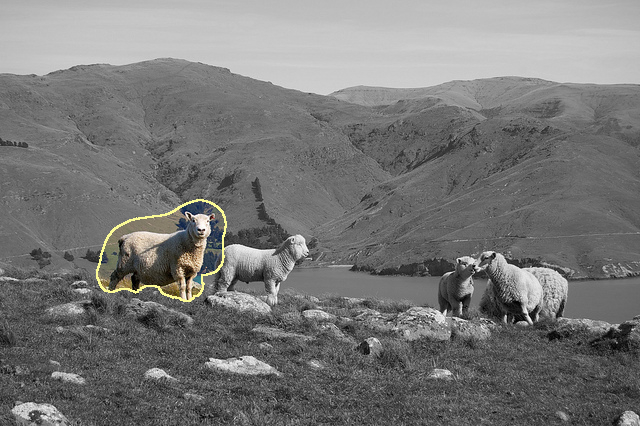
\includegraphics[scale=0.25]{figures/coco-experiment/parameter-tuning/sheep_r5/corrected-seg-with-data.png}}\hspace{1em}
\subfloat[Using $r=3$ ($(P+R)/2=0.94$)]{
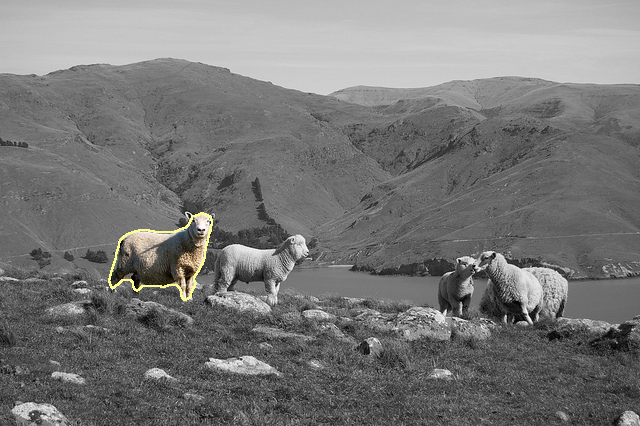
\includegraphics[scale=0.25]{figures/coco-experiment/parameter-tuning/sheep_r3/corrected-seg-with-data.png}}
\caption{\textbf{Parameter tuning.} The GFA was executed with the same set of parameters for all images, but we can recover better results by tuning the parameter for each image separately. In this example, the low scale of the image asks for a lower estimation radius. The precision plus recall average goes from $0.78$ to $0.94$ by using a radius of $3$ instead of $5$. }
\label{fig:coco-parameter-tuning}
\end{figure}
%
%
\subsection{Unsupervised binary segmentation}
The goal of this experiment is to illustrate the flexibility of the GFA with respect to the data fidelity term. In this experiment, we employed a Chan-Vese allike data term~\cite{chan01}, i.e., we penalize the square mean error between pixel intensity and the average foreground color (similarly for the background). We define the initial solution as an uniform collection of disks covering the image domain.

In this application, our strategy to avoid local minima is slightly different. We use a neighborhood of shapes composed by random perturbations of the initial contour and we allow evolution if and only if the previous energy value is reduced. This strategy lead to higher running times, but since the digital components are treated independently, we believe that running times can be greatly reduced by implementing a more agressive parallelization strategy, for example, using GPUs. 

The algorithm can evolve the contours in favor of contour completion or breaking them according to the relative weights given for the elastica and data terms. We show the results of some experiments in figure~\ref{fig:GF-chan-vese-alike}.

\begin{figure}
\center
\subfloat[Segmentation by grabcut]{
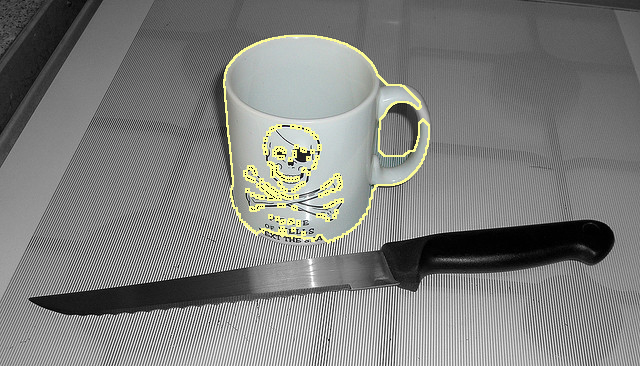
\includegraphics[scale=0.185]{figures/coco-experiment/completion/cup/gc-seg.png}\hspace{0.5em}
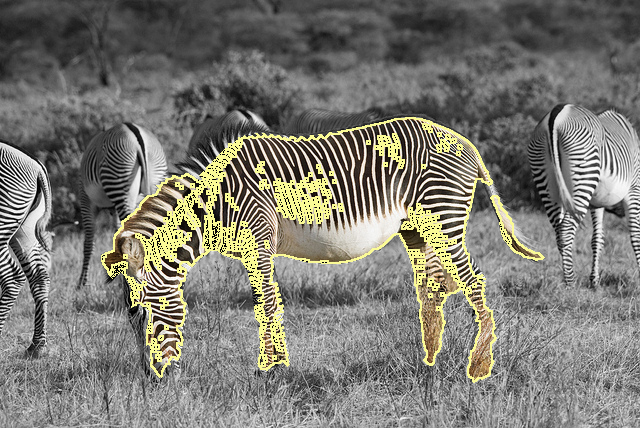
\includegraphics[scale=0.16]{figures/coco-experiment/completion/zebra/gc-seg.png}
\hspace{0.5em}
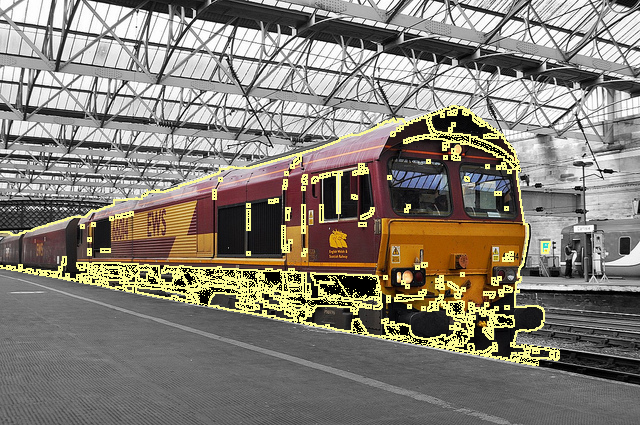
\includegraphics[scale=0.16]{figures/coco-experiment/completion/train/gc-seg.png}
}%

\subfloat[Segmentation corrected by GFA]{
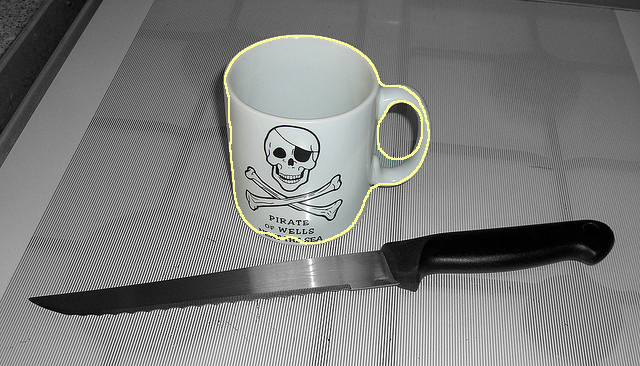
\includegraphics[scale=0.185]{figures/coco-experiment/completion/cup/corrected-seg-with-data.png}\hspace{0.5em}
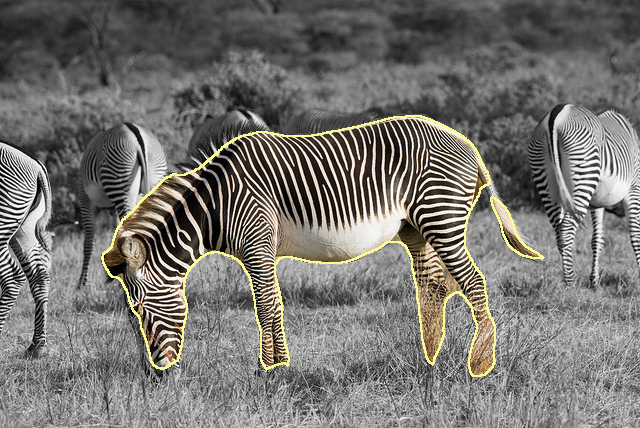
\includegraphics[scale=0.16]{figures/coco-experiment/completion/zebra/corrected-seg-with-data.png}
\hspace{0.5em}
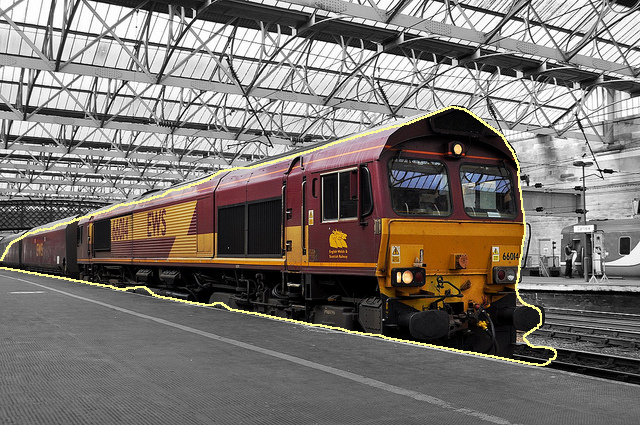
\includegraphics[scale=0.16]{figures/coco-experiment/completion/train/corrected-seg-with-data.png}
}%
\caption{\textbf{Contour completion.} The GFA favors connected components due to the completion effect of the elastica energy. That is particularly useful to avoid oversegmentation.}
\label{fig:coco-completion}
\end{figure}

\begin{figure}
\center
\subfloat[$22$ iterations ($52$s).]{
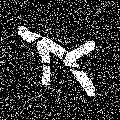
\includegraphics[scale=0.5]{figures/chan-vese-alike/branch/branch-noisy.png}
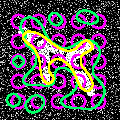
\includegraphics[scale=0.5]{figures/chan-vese-alike/branch/contours.png}
}\hspace{1em}%
\subfloat[$26$ iterations ($76$s).]{
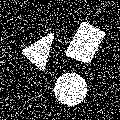
\includegraphics[scale=0.5]{figures/chan-vese-alike/simple-geometry/simple-geometry-noisy.png}
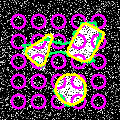
\includegraphics[scale=0.5]{figures/chan-vese-alike/simple-geometry/contours.png}
}%
\caption{\textbf{Chan-Vese alike data term.} The initial contour is highlighted in pink and the final contour in yellow. An intermediate contour is also highlighted in green. A proper parameter setting favors component completion (left) or component break (right). Images are $100\times100$. }
\label{fig:GF-chan-vese-alike}
\end{figure}



\section{Conclusion}

We presented a discrete shape evolution algorithm driven by the elastica energy. The GFA is built on recent results on the multigrid convergence of curvature and tangent estimators and its main step consists in to compute the minimum cut of candidate graphs. A candidate graph is constructed for each element in a neighborhood of shapes of the current digital set and its minimum cut gives a candidate shape. At each iteration, the GFA selects the candidate shape with lowest elastica energy. We have shown that our model can escape local minimum in the shape evolution problem by using a very simple neighborhood scheme of shapes. Indeed, our experiments converged to the shape of minimum elastica energy. 

Next, we presented some applications in image processing tasks. The GFA delivery contours with fewer inflection points, smoother tangent profiles and lower elastica energy than those produced from grabcut. That is done while keeping high values of precision and recall with respect to the Coco annotated images used in our experiments. Finally, we presented an unsupervised segmentation model based on the classical Chan-Vese data term, which demonstrate the flexibility of the model. 

One of the strengths of our model is that the curvature estimation is based on digital data solely and it is not attached to a curve model, which may restrict the curve evolution and pose technical difficults regarding its update. Secondly, the GFA is highly parallelizable. We believe that a GPU implementation will greatly reduce the running times of our algorithm for all presented applications. The bottleneck is in the minimum cut computation, as it is difficult to come up with a parallel implementation, but since the latter is computed along a thin band of the shape contour, we believe that this is a minor problem.

There are some possible paths for future work. Firstly, the graph construction part of the algorithm can be optimized. In the current version, the graph is constructed at every iteration, but most of the time, the graph structure changes very slightly and this can be used to optimize its construction. Secondly, we use a very rough neighborhood of shapes in the supervised segmentation problem, i.e., based on dilations and erosions of the initial shape. The contour completion property of the model can be better exploited by employing different neighborhoods. For example, we could alongate the initial shapes in regions of high curvature to obtain a stretched neighborhood of shapes. This could be particularly useful in the segmentation of thin and elongated objects such as blood vessels.


\printbibliography

\end{document}

